% =============================================================================
%  IV-2-9 — Бие даалт 1 тайлан
%  F.CSM302 Үйлдлийн систем, Бие даалт 1.  Хөрвүүлэгч: XeLaTeX (Overleaf: Menu → Compiler)
%  Энэ файлыг tools/build_docs.py бодит тест, туршилтын үр дүнгээс үүсгэсэн; шууд засаж болно.
% =============================================================================
\documentclass[12pt,a4paper]{article}
\usepackage{shutis}

% ---------------- Баримтын мэдээлэл (энд засна) ----------------
\newcommand{\DocTopic}{"Designing a Thread Pool. Programming Project 1 (7-р бүлэг), Worker activity"}
\newcommand{\DocCode}{IV-2-9}
\newcommand{\DocTeacher}{Г.Ганбат /F.CS10/}
\newcommand{\DocCity}{Улаанбаатар хот}
\newcommand{\DocYear}{2026 он}
\newcommand{\DocTeam}{%   \member{Овог.Нэр}{Оюутны код}
  \member{Ц.Номинжин}{B241940137}
  \member{Е.Айсауле}{B221940407}
  \member{Б.Балжинням}{B231940033}
  \member{М.Бат-Орших}{B200930061}
  \member{Г.Хулан}{B241940027}
  \member{Э.Энхсайхан}{B242270097}
}
\hypersetup{pdftitle={IV-2-9 — Бие даалт 1 тайлан}, pdfauthor={F.CSM302 IV-2-9 баг}}

\begin{document}
\makecover{ТАЙЛАН}

\section*{Хураангуй}
\addcontentsline{toc}{section}{Хураангуй}

\textbf{Асуудал.} Хүсэлт бүрт шинэ thread үүсгэх нь үүсгэх, устгах зардалтай бөгөөд нэгэн зэрэг ажиллах thread-ийн тоог хязгаарладаггүй. Thread pool нь цөөн worker thread-ийг урьдчилан үүсгэж, ажлыг дундын queue-ээр хуваарилна. Энэ queue-д client болон worker-ууд зэрэг хандах тул race condition үүсэх, ажилгүй worker CPU дэмий үрэх аюултай.

\textbf{Шийдэл.} Сурах бичгийн Programming Project 1-ийн POSIX хувилбарын дагуу C хэл, POSIX thread (pthreads), mutex lock болон counting semaphore ашиглан \code{pool\_init}, \code{pool\_submit}, \code{pool\_shutdown} API-тай thread pool хэрэгжүүлэв. Программ үйлдэл бүрээ микросекундын нарийвчлалтай JSON trace болгон гаргана. Браузерийн интерфейс уг программыг бодитоор ажиллуулж, багшийн оноосон "Worker activity" дүрслэлээр worker бүрийн idle, running, completed төлөв, queue-ийн дүүргэлт, татгалзлыг алхам алхмаар харуулна.

\textbf{Туршилт.} Программыг 29 автомат тестээр (номын жишээ, үндсэн, захын, буруу оролт) шалгав. Тест бүрийн trace-ийг C кодоос хараат бус Python шалгагчаар дахин шалгаж, ThreadSanitizer-ээр race condition хайв. Worker-ийн тоо, queue-ийн багтаамж, дүүрэх үеийн бодлогын нөлөөг гурван туршилтаар хэмжив.

\textbf{Гол үр дүн.} 29/29 тест амжилттай. Бүх ажиллуулалтад task бүр яг нэг удаа гүйцэтгэгдэж, queue FIFO дарааллаар ажиллаж, багтаамжаас хэтрээгүй. ThreadSanitizer race илрүүлээгүй. 40 task-ийн ачаалалд worker-ийн тоог 1-ээс 16 болгоход нийт хугацаа 8377 мс-ээс 647 мс болж 13.0 дахин хурдассан.

\clearpage

\tableofcontents
\clearpage

% ======================================================================
\section{Удиртгал}

\subsection{Зорилго}

Сурах бичгийн 7-р бүлгийн Programming Project 1 "Designing a Thread Pool"-ийг хэрэгжүүлж, хэрэглэгч worker-ийн тоо, queue-ийн багтаамж, ажлын параметрийг өөрчилж турших боломжтой программ бүтээх. Программын ажиллагааг багшийн оноосон "Worker activity" дүрслэлээр харуулж, хэрэгжилт болон туршилтын үр дүнг баримтжуулах.

\subsection{Ач холбогдол}

Thread pool нь вэб сервер, өгөгдлийн сангийн сервер, Java-ийн \code{ExecutorService}, Linux kernel-ийн \code{workqueue} зэрэг олон системийн үндэс юм. Энэ төсөл нь mutex, semaphore, bounded buffer (producer-consumer) ойлголтыг нэг бодит программд нэгтгэнэ: task өгөгч client нь producer, worker-ууд нь consumer болно. Thread-үүдийн ажиллагаа нүдэнд харагддаггүй тул worker бүрийн төлөвийг хугацааны тэнхлэг дээр дүрслэх нь ойлголтыг ихээхэн хөнгөвчилнө.

\subsection{Хамрах хүрээ}

\begin{itemize}
  \item C хэл дээрх thread pool: тойрог массив queue, \code{pthread\_mutex}, \code{sem\_t} semaphore, worker thread (сурах бичгийн үндсэн шаардлага).
  \item Номын API-г өөрчлөлтгүй хадгалж, worker-ийн тоо болон queue-ийн багтаамжийг тохируулах өргөтгөл.
  \item Оролтыг шалгах, үйлдэл бүрийг JSON trace болгон хэвлэх, ажиллаж дууссаны дараа 8 инвариант шалгах.
  \item Бодит программтай холбогдсон браузерийн интерфейс: тохиргоо, Worker activity дүрслэл, timeline, үйл явдлын бүртгэл.
  \item Автомат тест, ThreadSanitizer, CI, хэрэглэгчийн ба operational гарын авлага (Manual).
\end{itemize}

Java хувилбар (номонд сонголтоор өгсөн), task-ийн priority, worker-ийн тоог ажиллах явцад динамикаар өөрчлөх хамрах хүрээнд ороогүй.

% ======================================================================
\section{Сурах бичгийн шаардлага}

\subsection{Programming Project 1-ийн үндсэн шаардлага}

Сурах бичгийн (Silberschatz, Galvin, Gagne, \textit{Operating System Concepts}, 10-р хэвлэл) 7-р бүлгийн Project 1 нь client-ийн өгсөн ажлыг thread pool-ийн worker-уудаар гүйцэтгэхийг шаардана. POSIX хувилбарын шаардлага:

\begin{enumerate}
  \item \code{pool\_init()} нь worker thread-үүдийг эхэнд нь үүсгэж, mutex болон semaphore-ийг эхлүүлнэ.
  \item \code{pool\_submit()} нь функц болон өгөгдлийг \code{task} бүтэц болгож \code{enqueue()}-ээр queue-д хийнэ. Queue массив бөгөөд дүүрсэн бол 1, амжилттай бол 0 буцаана.
  \item \code{worker()} нь ажил ирэхийг semaphore дээр хүлээж, \code{dequeue()}-ээр авсан task-ийг \code{execute()}-ээр гүйцэтгэнэ.
  \item Queue-д хандах бүх үйлдлийг mutex lock-оор хамгаална.
  \item \code{pool\_shutdown()} нь worker-уудыг зогсоож \code{pthread\_join()} хийнэ. Номын \code{client.c} жишээ ажиллах ёстой.
\end{enumerate}

\subsection{Багшийн нэмэлт шаардлага}

Бие даалт 1-ийн удирдамжаар дараах шаардлага нэмэгдэнэ: оролт, параметрийг өөрчилж дахин турших; буруу болон захын оролтыг шалгаж ойлгомжтой мэдээлэх; тохиргоог солих, дахин ажиллуулах, reset хийх; оноосон "Worker activity" UI-г бодит ажиллагаатай холбох; номын болон нэмэлт туршилтаар зөв ажиллагааг нотлох; Manual-ын дагуу өөр компьютерт ажиллуулах боломжтой байх; GitHub repository, README, Release/Tag. Хуваарилалтын файлд 9-р сэдвийн хүрэх үр дүнг "Worker-ийн тоо, task queue, ажлын параметрийг өөрчилж, worker бүрийн idle, running, completed төлөвийг хугацааны явцад харуулна" гэж тодорхойлсон.

\subsection{Шаардлагын хангалт}

\begin{longtable}{|P{0.420}|P{0.580}|}
\caption{Шаардлага ба хэрэгжсэн газар}\label{tab:req}\\
\hline
\rowcolor{tablehead} \textbf{Шаардлага} & \textbf{Хэрэгжилт} \\ \hline
\endfirsthead
\hline
\rowcolor{tablehead} \textbf{Шаардлага} & \textbf{Хэрэгжилт} \\ \hline
\endhead
\code{pool\_init}: thread, mutex, semaphore & \code{src/threadpool.c}: \code{pool\_init()} (3 worker, queue 10), \code{pool\_init\_ex(n, cap)} \\ \hline
\code{pool\_submit}, массив queue, дүүрвэл 1 & Тойрог массив, \code{POOL\_OK=0}, \code{POOL\_FULL=1} \\ \hline
\code{worker}: semaphore дээр хүлээх & \code{sem\_wait(work\_available)} → \code{dequeue()} → \code{execute()} \\ \hline
Queue-г mutex-ээр хамгаалах & \code{pthread\_mutex\_t qmutex} \\ \hline
\code{pool\_shutdown}, \code{pthread\_join} & Shutdown флаг + worker бүрт нэг sem\_post, үлдсэн task-уудыг гүйцээгээд гарна \\ \hline
Номын \code{client.c} & \code{examples/client.c}, тест T1 \\ \hline
Параметр өөрчилж дахин турших, reset & Интерфейсийн тохиргоо, Ажиллуулах/Reset/Анхдагч, бэлэн тест; CLI сонголтууд \\ \hline
Буруу оролт шалгах & C программ (exit 2 + тайлбар), сервер (HTTP 400), UI (улаан талбар) \\ \hline
Worker activity, бодит ажиллагаатай холбох & Бодит C программын trace-ээр worker карт, queue, timeline зурна \\ \hline
Нэмэлт туршилт & 29 автомат тест, хараат бус trace шалгагч, ThreadSanitizer, 3 туршилт, CI \\ \hline
\end{longtable}

% ======================================================================
\section{Онолын үндэс}

\subsection{Thread pool}

Thread pool нь эхлэхдээ тогтмол тооны thread үүсгэж, тэднийг pool-д хүлээлгэнэ. Ирсэн ажил queue-д орж, чөлөөтэй thread түүнийг авч гүйцэтгээд дахин pool руу буцна (номын 4.5.1). Давуу тал нь: байгаа thread-ээр үйлчлэх нь шинэ thread үүсгэхээс хурдан; нэгэн зэрэг ажиллах thread-ийн тоо хязгаарлагдмал тул систем хэт ачаалагдахгүй; ажлыг гүйцэтгэх механизмаас тусгаарласан тул хуваарилах стратегийг тусад нь өөрчилж болно.

\subsection{Critical section ба race condition}

Хэд хэдэн thread нэг дундын өгөгдлийг зэрэг өөрчлөх үед үр дүн нь гүйцэтгэлийн дараалалаас хамаарах нөхцөлийг race condition гэнэ. Queue-д task нэмэх нь "\code{queue[tail] = t}", "\code{tail = (tail + 1) \% cap}", "\code{count++}" гэсэн хэд хэдэн алхмаас бүрдэх critical section юм. Хоёр worker зэрэг dequeue хийвэл нэг task-ийг давхар авч, нөгөөг алгасах аюултай. Critical section-ийн шийдэл нь харилцан гадуурхал (mutual exclusion), ахиц (progress), хязгаартай хүлээлт (bounded waiting) гэсэн гурван шаардлагыг хангах ёстой.

\subsection{Mutex lock}

Mutex нь нэг мөчид зөвхөн нэг thread-д critical section-д орох эрх олгоно (\code{pthread\_mutex\_lock/unlock}). Цоож барьсан thread л queue-г өөрчлөх тул \code{head}, \code{tail}, \code{count} зөрөхгүй. Цоожийг аль болох богино хугацаанд барих ёстой: task-ийг гүйцэтгэх хугацаанд барьвал worker-ууд дараалж ажиллан pool утгагүй болно.

\subsection{Semaphore}

Semaphore нь бүхэл тоон утгатай хувьсагч бөгөөд зөвхөн хоёр атомар үйлдлээр хандана. \code{wait()} (POSIX: \code{sem\_wait}) утгыг 1-ээр хасна; утга 0 байвал thread блоклогдож хүлээнэ. \code{signal()} (\code{sem\_post}) утгыг 1-ээр нэмж, хүлээж буй thread байвал нэгийг сэрээнэ. Thread pool-д counting semaphore-ийн утга нь queue дахь task-ийн тоотой тэнцүү: ажилгүй worker \code{sem\_wait} дээр унтаж, CPU үрэхгүй (busy waiting байхгүй). Номд unnamed semaphore (\code{sem\_init(\&sem, 0, 0)}) ашиглахыг зөвлөсөн.

\subsection{Bounded buffer ба тойрог queue}

Thread pool-ийн queue нь номын 7.1.1 хэсгийн bounded buffer бодлогын нэг хэлбэр. Номын шийдэл \code{mutex}, \code{empty}, \code{full} гурван синхрончлолын хувьсагч ашигладаг (номын Зураг 7.1–7.2):

\par\noindent\begin{minipage}{\linewidth}\setlength{\topsep}{1pt}\setlength{\partopsep}{0pt}
\captionof{codeblock}{Consumer-ийн бүтэц (номын Зураг 7.2)}\label{lst:book}
\begin{Verbatim}[commandchars=\\\{\}]
\PY{k}{while}\PY{+w}{ }\PY{p}{(}\PY{n+nb}{true}\PY{p}{)}\PY{+w}{ }\PY{p}{\PYZob{}}
\PY{+w}{   }\PY{n}{wait}\PY{p}{(}\PY{n}{full}\PY{p}{)}\PY{p}{;}
\PY{+w}{   }\PY{n}{wait}\PY{p}{(}\PY{n}{mutex}\PY{p}{)}\PY{p}{;}
\PY{+w}{   }\PY{c+cm}{/* remove an item from buffer to next\PYZus{}consumed */}
\PY{+w}{   }\PY{n}{signal}\PY{p}{(}\PY{n}{mutex}\PY{p}{)}\PY{p}{;}
\PY{+w}{   }\PY{n}{signal}\PY{p}{(}\PY{n}{empty}\PY{p}{)}\PY{p}{;}
\PY{+w}{   }\PY{c+cm}{/* consume the item in next\PYZus{}consumed */}
\PY{p}{\PYZcb{}}
\end{Verbatim}
\end{minipage}

Thread pool-д worker нь consumer бөгөөд \code{full}-ийн үүргийг \code{work\_available} semaphore гүйцэтгэнэ. Харин \code{empty}-ийн оронд дүүрсэн queue-д client-ийг блоклохгүйгээр шууд 1 буцаадаг нь номын \code{pool\_submit()}-ийн тодорхойлолт юм. Queue нь \code{cap} нүдтэй массив, хоёр заагчтай: \code{tail} нь дараагийн тавих нүд, \code{head} нь дараагийн авах нүд. Заагч бүр \code{(i + 1) \% cap}-ээр урагшилж, сүүлийн нүдний дараа 0 руу эргэнэ. Иймээс анх орсон task анх гүйцэтгэгдэнэ (FIFO).

\subsection{Thread-ийг зогсоох}

Номд \code{pthread\_cancel()}-ийг санал болгосон (\code{sem\_wait()} нь cancellation point). Гэвч deferred cancellation нь task ажиллаж байх үед \code{nanosleep} зэрэг cancellation point дээр thread-ийг тасалж, task-ийг дутуу орхих, барьсан нөөцийг суллахгүй байх эрсдэлтэй (номын 4.6.3). Тиймээс хамтран зогсох (cooperative) аргыг сонгов: shutdown флаг тавиад worker бүрт нэг \code{sem\_post} илгээнэ. Энэ нь API-ийн "бүх task дууссаны дараа зогсоно" гэсэн тайлбартай нийцнэ.

\subsection{Invariant}

Зөв синхрончлолтой ажиллалтын төгсгөлд "хүлээн авсан = гүйцэтгэсэн", "task бүр яг 1 удаа ажилласан", "нэгэн зэрэг ажилласан task ≤ worker-ийн тоо", "queue-ийн урт ≤ багтаамж" гэсэн тэнцэл үргэлж биелнэ. Программ төгсгөлд нь эдгээрийг шалгаж (\code{VERIFY: OK}), тест болон интерфейс зөв ажиллагааны нотолгоо болгон ашиглана.

% ======================================================================
\section{Системийн зохиомж}

\subsection{Бүрэлдэхүүн хэсгүүд}

Систем гурван хэсгээс бүрдэнэ (Зураг \ref{fig:arch}): синхрончлолыг бодитоор гүйцэтгэдэг C программ (core), түүнийг ажиллуулж trace-ийг дамжуулдаг Python сервер, trace-ийг дүрсэлдэг браузерийн интерфейс.

\begin{figure}[H]
\centering
\begin{tikzpicture}[node distance=1.15cm, box/.append style={text width=3.55cm}]
  \node[box] (core) {\textbf{C core}\\\code{threadpool\_sim}\\pthreads, mutex,\\semaphore, queue};
  \node[box, right=of core] (srv) {\textbf{Python сервер}\\\code{/api/run}: шалгах,\\\code{subprocess}, JSON\\trace буцаах};
  \node[box, right=of srv] (ui) {\textbf{Browser}\\\code{index.html}\\Worker activity,\\queue, timeline};
  \draw[flow] (core) -- node[lbl, above]{stdout} node[lbl, below]{JSON trace} (srv);
  \draw[flow] (srv) -- node[lbl, above]{HTTP} node[lbl, below]{JSON} (ui);
  \draw[flow] (ui.south) -- ++(0,-0.6) -| node[lbl, pos=0.25, below]{тохиргоо (JSON) $\rightarrow$ CLI аргумент} (core.south);
\end{tikzpicture}
\caption{Системийн бүрэлдэхүүн ба өгөгдлийн урсгал}\label{fig:arch}
\end{figure}

Core-ийн дотор client thread task-уудыг queue-д хийж, worker-ууд semaphore-оор сэрж авна (Зураг \ref{fig:pool}).

\begin{figure}[H]
\centering
\begin{tikzpicture}[font=\small]
  \node[box, text width=2.7cm, minimum height=1.35cm] (sub) at (0,0) {\code{pool\_submit()}\\lock $\rightarrow$ enqueue\\$\rightarrow$ unlock};
  \node[draw=headblue!60, fill=headblue!55, minimum size=0.66cm, inner sep=0pt, text=white, font=\scriptsize\ttfamily] (s0) at (3.25,0) {T3};
  \node[draw=headblue!60, fill=headblue!55, minimum size=0.66cm, inner sep=0pt, text=white, font=\scriptsize\ttfamily] (s1) at (4.07,0) {T4};
  \node[draw=headblue!60, fill=headblue!55, minimum size=0.66cm, inner sep=0pt, text=white, font=\scriptsize\ttfamily] (s2) at (4.89,0) {T5};
  \node[draw=black!35, dashed, minimum size=0.66cm, inner sep=0pt] (s3) at (5.71,0) {};
  \node[draw=black!35, dashed, minimum size=0.66cm, inner sep=0pt] (s4) at (6.53,0) {};
  \node[draw=black!25, rounded corners=5pt, fit=(s0)(s4), inner xsep=6pt, inner ysep=9pt] (q) {};
  \node[font=\small\bfseries, above=1pt of q] {Тойрог queue (\code{qmutex})};
  \node[font=\scriptsize, below=0pt of s0] {head};
  \node[font=\scriptsize, below=0pt of s3] {tail};
  \node[draw=yellow!45!black!45, fill=yellow!8, rounded corners=9pt, align=center, font=\scriptsize, inner sep=4pt]
       (sem) at (4.9,-2.05) {\code{sem work\_available}\\= queue дахь task-ийн тоо};
  \node[box, text width=3.4cm, minimum height=0.9cm, font=\scriptsize, fill=headblue!6] (w0) at (10.75,1.25) {\textbf{Worker 0}\\running T2 (mutex-ээс гадна)};
  \node[box, text width=3.4cm, minimum height=0.9cm, font=\scriptsize, fill=headblue!6] (w1) at (10.75,0) {\textbf{Worker 1}\\sem\_wait $\rightarrow$ dequeue $\rightarrow$ execute};
  \node[box, text width=3.4cm, minimum height=0.9cm, font=\scriptsize] (w2) at (10.75,-1.25) {\textbf{Worker N$-$1}\\idle: sem\_wait дээр блоклогдсон};
  \draw[flow] (sub) -- (q);
  \draw[flow] (q.east) -- node[lbl, above]{dequeue} (w1.west);
  \draw[flow, dashed, draw=yellow!40!black!70] (sub.south) |- node[lbl, pos=0.75, above, text=yellow!40!black!80]{\code{sem\_post}} (sem.west);
  \draw[flow, dashed, draw=yellow!40!black!70] (sem.east) -- node[lbl, below right, text=yellow!40!black!80]{сэрээнэ} (w2.west);
\end{tikzpicture}
\caption{Pool доторх урсгал: submit → queue → semaphore → worker}\label{fig:pool}
\end{figure}

\subsection{Өгөгдлийн урсгал}

\begin{enumerate}
  \item Хэрэглэгч тохиргоо хэсэгт worker, queue, бодлого, task-ийн тоо, хугацаа, ирэх зай, seed-ийг сонгох эсвэл task жагсаалт оруулаад \textbf{Ажиллуулах} дарна.
  \item Browser \code{POST /api/run} хүсэлт илгээнэ. Сервер утгуудыг CLI аргумент болгож \code{build/threadpool\_sim}-ийг ажиллуулна. Буруу утгыг C программ өөрөө шалгаж, exit 2 + тайлбар буцаавал сервер HTTP 400 болгон дамжуулна.
  \item Core pool-ийг эхлүүлж, task бүрийг тогтоосон агшинд submit хийн, worker-ууд бодитоор гүйцэтгэнэ. Үйлдэл бүр санах ойн trace-д бүртгэгдэнэ. Shutdown-ы дараа 8 инвариант шалгаад бүх trace-ийг JSON болгон stdout руу хэвлэнэ.
  \item Browser JSON-ийг хүлээн авч worker карт, queue, timeline, бүртгэлийг зурж, playback-аар тоглуулна. Trace-ийг файлд хадгалж, дараа нь сервергүйгээр дахин үзэж болно.
\end{enumerate}

\subsection{Үйлдлийн (event) формат}

Trace-ийн үйлдэл бүр нэг мөр бөгөөд тухайн агшны queue-ийн уртыг агуулна (Хүснэгт \ref{tab:ev}).

\begin{table}[H]
\centering
\caption{JSON үйлдлийн талбарууд}\label{tab:ev}
\begin{tabular}{|P{0.220}|P{0.780}|}
\hline
\rowcolor{tablehead} \textbf{Талбар} & \textbf{Утга} \\ \hline
\code{t} & \code{pool\_init}-ээс хойшх хугацаа (микросекунд) \\ \hline
\code{type} & \code{POOL\_INIT}, \code{IDLE}, \code{SUBMIT}, \code{REJECT}, \code{START}, \code{END}, \code{SHUTDOWN}, \code{WORKER\_EXIT} \\ \hline
\code{w} & worker-ийн дугаар (0-ээс), хамааралгүй бол −1 \\ \hline
\code{task} & task-ийн дугаар, хамааралгүй бол −1 \\ \hline
\code{q} & үйлдлийн дараах queue-ийн урт \\ \hline
\code{summary} & \code{submitted}, \code{rejected}, \code{completed}, \code{avg\_wait\_ms}, \code{makespan\_ms}, \code{utilization\_pct}, \code{per\_worker} \\ \hline
\code{verify} & \code{ok} ба 8 шалгалтын нэр, үр дүн, тайлбар \\ \hline
\end{tabular}
\end{table}

Жишээ мөр:

\par\noindent\begin{minipage}{\linewidth}\setlength{\topsep}{1pt}\setlength{\partopsep}{0pt}
\begin{Verbatim}[commandchars=\\\{\}]
\PY{p}{\PYZob{}}\PY{n+nt}{\PYZdq{}t\PYZdq{}}\PY{p}{:}\PY{l+m+mi}{94}\PY{p}{,}\PY{n+nt}{\PYZdq{}type\PYZdq{}}\PY{p}{:}\PY{l+s+s2}{\PYZdq{}SUBMIT\PYZdq{}}\PY{p}{,}\PY{n+nt}{\PYZdq{}w\PYZdq{}}\PY{p}{:}\PY{l+m+mi}{\PYZhy{}1}\PY{p}{,}\PY{n+nt}{\PYZdq{}task\PYZdq{}}\PY{p}{:}\PY{l+m+mi}{0}\PY{p}{,}\PY{n+nt}{\PYZdq{}q\PYZdq{}}\PY{p}{:}\PY{l+m+mi}{1}\PY{p}{\PYZcb{},}
\PY{p}{\PYZob{}}\PY{n+nt}{\PYZdq{}t\PYZdq{}}\PY{p}{:}\PY{l+m+mi}{122}\PY{p}{,}\PY{n+nt}{\PYZdq{}type\PYZdq{}}\PY{p}{:}\PY{l+s+s2}{\PYZdq{}START\PYZdq{}}\PY{p}{,}\PY{n+nt}{\PYZdq{}w\PYZdq{}}\PY{p}{:}\PY{l+m+mi}{1}\PY{p}{,}\PY{n+nt}{\PYZdq{}task\PYZdq{}}\PY{p}{:}\PY{l+m+mi}{0}\PY{p}{,}\PY{n+nt}{\PYZdq{}q\PYZdq{}}\PY{p}{:}\PY{l+m+mi}{0}\PY{p}{\PYZcb{}}
\end{Verbatim}
\end{minipage}

Цагийг trace-ийн mutex дотор авдаг тул массивын дараалал хугацааны дараалалтай давхцана. \code{SUBMIT}, \code{START}-ийг queue-ийн mutex дор бүртгэдэг тул бүртгэсэн \code{q} нь бодит queue-ийн урттай яг тэнцүү.

\subsection{Хязгаар ба хамгаалалт}

C программ: worker 1-64, queue 1-4096, task 1-10000, хугацаа 1-60000 мс, ирэх зай 0-60000 мс. Сервер нэг ажиллуулалтад интерфейсээс 2000-аас олон task, ойролцоогоор 60 секундээс урт ажлыг хүлээж авахгүй, 120 секундэд дуусаагүй процессыг зогсооно, зөвхөн 127.0.0.1 хаягаас хүсэлт хүлээн авна.

% ======================================================================
\section{Хэрэгжилт}

\subsection{Хэл, сан, орчин}

\begin{table}[H]
\centering
\caption{Ашигласан технологи}\label{tab:tech}
\begin{tabular}{|P{0.220}|P{0.780}|}
\hline
\rowcolor{tablehead} \textbf{Хэсэг} & \textbf{Технологи} \\ \hline
Core & C11 (gcc/clang, \code{-O2 -Wall -Wextra -pthread}), POSIX threads, POSIX semaphore (macOS дээр \code{dispatch\_semaphore}) \\ \hline
Сервер & Python 3 стандарт сан (\code{http.server}, \code{subprocess}), нэмэлт сангүй \\ \hline
Интерфейс & HTML, CSS, JavaScript, SVG; гадны сан, CDN ашиглаагүй \\ \hline
Тест & POSIX shell (\code{tests/run\_tests.sh}), Python 3 (\code{tests/verify\_trace.py}), ThreadSanitizer \\ \hline
CI & GitHub Actions (ubuntu-latest, macos-latest) \\ \hline
\end{tabular}
\end{table}

\subsection{C core: queue}

Номын API-г хадгалж, queue-г тойрог массиваар хэрэгжүүлэв. Функцууд \code{qmutex} барьсан үед л дуудагдана.

\par\noindent\begin{minipage}{\linewidth}\setlength{\topsep}{1pt}\setlength{\partopsep}{0pt}
\captionof{codeblock}{\code{enqueue} ба \code{dequeue} (src/threadpool.c)}\label{lst:queue}
\begin{Verbatim}[commandchars=\\\{\}]
\PY{k}{static}\PY{+w}{ }\PY{k+kt}{int}\PY{+w}{ }\PY{n+nf}{enqueue}\PY{p}{(}\PY{n}{task}\PY{+w}{ }\PY{n}{t}\PY{p}{)}
\PY{p}{\PYZob{}}
\PY{+w}{    }\PY{k}{if}\PY{+w}{ }\PY{p}{(}\PY{n}{qcount}\PY{+w}{ }\PY{o}{=}\PY{o}{=}\PY{+w}{ }\PY{n}{qcap}\PY{p}{)}\PY{+w}{ }\PY{k}{return}\PY{+w}{ }\PY{l+m+mi}{1}\PY{p}{;}
\PY{+w}{    }\PY{n}{queue}\PY{p}{[}\PY{n}{qtail}\PY{p}{]}\PY{+w}{ }\PY{o}{=}\PY{+w}{ }\PY{n}{t}\PY{p}{;}
\PY{+w}{    }\PY{n}{qtail}\PY{+w}{ }\PY{o}{=}\PY{+w}{ }\PY{p}{(}\PY{n}{qtail}\PY{+w}{ }\PY{o}{+}\PY{+w}{ }\PY{l+m+mi}{1}\PY{p}{)}\PY{+w}{ }\PY{o}{\PYZpc{}}\PY{+w}{ }\PY{n}{qcap}\PY{p}{;}
\PY{+w}{    }\PY{n}{qcount}\PY{o}{+}\PY{o}{+}\PY{p}{;}
\PY{+w}{    }\PY{k}{return}\PY{+w}{ }\PY{l+m+mi}{0}\PY{p}{;}
\PY{p}{\PYZcb{}}

\PY{k}{static}\PY{+w}{ }\PY{n}{task}\PY{+w}{ }\PY{n+nf}{dequeue}\PY{p}{(}\PY{k+kt}{void}\PY{p}{)}
\PY{p}{\PYZob{}}
\PY{+w}{    }\PY{n}{task}\PY{+w}{ }\PY{n}{t}\PY{+w}{ }\PY{o}{=}\PY{+w}{ }\PY{n}{queue}\PY{p}{[}\PY{n}{qhead}\PY{p}{]}\PY{p}{;}
\PY{+w}{    }\PY{n}{qhead}\PY{+w}{ }\PY{o}{=}\PY{+w}{ }\PY{p}{(}\PY{n}{qhead}\PY{+w}{ }\PY{o}{+}\PY{+w}{ }\PY{l+m+mi}{1}\PY{p}{)}\PY{+w}{ }\PY{o}{\PYZpc{}}\PY{+w}{ }\PY{n}{qcap}\PY{p}{;}
\PY{+w}{    }\PY{n}{qcount}\PY{o}{\PYZhy{}}\PY{o}{\PYZhy{}}\PY{p}{;}
\PY{+w}{    }\PY{k}{return}\PY{+w}{ }\PY{n}{t}\PY{p}{;}
\PY{p}{\PYZcb{}}
\end{Verbatim}
\end{minipage}

\subsection{C core: worker}

Worker \code{sem\_wait}-ээр ажил хүлээж, mutex дор dequeue хийгээд, task-ийг mutex-ийн \textbf{гадна} гүйцэтгэнэ (Код \ref{lst:worker}).

\par\noindent\begin{minipage}{\linewidth}\setlength{\topsep}{1pt}\setlength{\partopsep}{0pt}
\captionof{codeblock}{Worker thread-ийн функц (src/threadpool.c)}\label{lst:worker}
\begin{Verbatim}[commandchars=\\\{\}]
\PY{k}{static}\PY{+w}{ }\PY{k+kt}{void}\PY{+w}{ }\PY{o}{*}\PY{n+nf}{worker}\PY{p}{(}\PY{k+kt}{void}\PY{+w}{ }\PY{o}{*}\PY{n}{param}\PY{p}{)}
\PY{p}{\PYZob{}}
\PY{+w}{    }\PY{n}{worker\PYZus{}info}\PY{+w}{ }\PY{o}{*}\PY{n}{me}\PY{+w}{ }\PY{o}{=}\PY{+w}{ }\PY{n}{param}\PY{p}{;}

\PY{+w}{    }\PY{k}{for}\PY{+w}{ }\PY{p}{(}\PY{p}{;}\PY{p}{;}\PY{p}{)}\PY{+w}{ }\PY{p}{\PYZob{}}
\PY{+w}{        }\PY{n}{trace}\PY{p}{(}\PY{n}{EV\PYZus{}WORKER\PYZus{}IDLE}\PY{p}{,}\PY{+w}{ }\PY{n}{me}\PY{o}{\PYZhy{}}\PY{o}{\PYZgt{}}\PY{n}{id}\PY{p}{,}\PY{+w}{ }\PY{l+m+mi}{\PYZhy{}1}\PY{p}{,}\PY{+w}{ }\PY{l+m+mi}{\PYZhy{}1}\PY{p}{)}\PY{p}{;}
\PY{+w}{        }\PY{n}{psem\PYZus{}wait}\PY{p}{(}\PY{o}{\PYZam{}}\PY{n}{work\PYZus{}available}\PY{p}{)}\PY{p}{;}\PY{+w}{  }\PY{c+cm}{/* ажил (эсвэл shutdown) хүлээнэ */}

\PY{+w}{        }\PY{n}{pthread\PYZus{}mutex\PYZus{}lock}\PY{p}{(}\PY{o}{\PYZam{}}\PY{n}{qmutex}\PY{p}{)}\PY{p}{;}
\PY{+w}{        }\PY{k}{if}\PY{+w}{ }\PY{p}{(}\PY{n}{qcount}\PY{+w}{ }\PY{o}{=}\PY{o}{=}\PY{+w}{ }\PY{l+m+mi}{0}\PY{+w}{ }\PY{o}{\PYZam{}}\PY{o}{\PYZam{}}\PY{+w}{ }\PY{n}{shutting\PYZus{}down}\PY{p}{)}\PY{+w}{ }\PY{p}{\PYZob{}}\PY{+w}{  }\PY{c+cm}{/* queue хоосон + shutdown → гарна */}
\PY{+w}{            }\PY{n}{pthread\PYZus{}mutex\PYZus{}unlock}\PY{p}{(}\PY{o}{\PYZam{}}\PY{n}{qmutex}\PY{p}{)}\PY{p}{;}
\PY{+w}{            }\PY{k}{break}\PY{p}{;}
\PY{+w}{        }\PY{p}{\PYZcb{}}
\PY{+w}{        }\PY{n}{task}\PY{+w}{ }\PY{n}{t}\PY{+w}{ }\PY{o}{=}\PY{+w}{ }\PY{n}{dequeue}\PY{p}{(}\PY{p}{)}\PY{p}{;}
\PY{+w}{        }\PY{n}{trace}\PY{p}{(}\PY{n}{EV\PYZus{}START}\PY{p}{,}\PY{+w}{ }\PY{n}{me}\PY{o}{\PYZhy{}}\PY{o}{\PYZgt{}}\PY{n}{id}\PY{p}{,}\PY{+w}{ }\PY{n}{t}\PY{p}{.}\PY{n}{id}\PY{p}{,}\PY{+w}{ }\PY{n}{qcount}\PY{p}{)}\PY{p}{;}
\PY{+w}{        }\PY{n}{pthread\PYZus{}mutex\PYZus{}unlock}\PY{p}{(}\PY{o}{\PYZam{}}\PY{n}{qmutex}\PY{p}{)}\PY{p}{;}

\PY{+w}{        }\PY{n}{execute}\PY{p}{(}\PY{n}{t}\PY{p}{.}\PY{n}{function}\PY{p}{,}\PY{+w}{ }\PY{n}{t}\PY{p}{.}\PY{n}{data}\PY{p}{)}\PY{p}{;}\PY{+w}{  }\PY{c+cm}{/* critical section\PYZhy{}оос ГАДНА */}

\PY{+w}{        }\PY{n}{pthread\PYZus{}mutex\PYZus{}lock}\PY{p}{(}\PY{o}{\PYZam{}}\PY{n}{qmutex}\PY{p}{)}\PY{p}{;}
\PY{+w}{        }\PY{n}{completed}\PY{o}{+}\PY{o}{+}\PY{p}{;}
\PY{+w}{        }\PY{n}{per\PYZus{}worker\PYZus{}completed}\PY{p}{[}\PY{n}{me}\PY{o}{\PYZhy{}}\PY{o}{\PYZgt{}}\PY{n}{id}\PY{p}{]}\PY{o}{+}\PY{o}{+}\PY{p}{;}
\PY{+w}{        }\PY{n}{trace}\PY{p}{(}\PY{n}{EV\PYZus{}END}\PY{p}{,}\PY{+w}{ }\PY{n}{me}\PY{o}{\PYZhy{}}\PY{o}{\PYZgt{}}\PY{n}{id}\PY{p}{,}\PY{+w}{ }\PY{n}{t}\PY{p}{.}\PY{n}{id}\PY{p}{,}\PY{+w}{ }\PY{n}{qcount}\PY{p}{)}\PY{p}{;}
\PY{+w}{        }\PY{n}{pthread\PYZus{}mutex\PYZus{}unlock}\PY{p}{(}\PY{o}{\PYZam{}}\PY{n}{qmutex}\PY{p}{)}\PY{p}{;}
\PY{+w}{    }\PY{p}{\PYZcb{}}

\PY{+w}{    }\PY{n}{trace}\PY{p}{(}\PY{n}{EV\PYZus{}WORKER\PYZus{}EXIT}\PY{p}{,}\PY{+w}{ }\PY{n}{me}\PY{o}{\PYZhy{}}\PY{o}{\PYZgt{}}\PY{n}{id}\PY{p}{,}\PY{+w}{ }\PY{l+m+mi}{\PYZhy{}1}\PY{p}{,}\PY{+w}{ }\PY{l+m+mi}{\PYZhy{}1}\PY{p}{)}\PY{p}{;}
\PY{+w}{    }\PY{k}{return}\PY{+w}{ }\PY{n+nb}{NULL}\PY{p}{;}
\PY{p}{\PYZcb{}}
\end{Verbatim}
\end{minipage}

Гол шийдлүүд:

\begin{itemize}
  \item \code{sem\_wait} нь mutex-ээс гадна байна. Mutex барьсан чигээр блоклогдвол client submit хийж чадахгүй тул deadlock болно.
  \item \code{execute()}-ийг mutex-ийг суллаад дуудна. Ингэснээр N worker зэрэг ажиллана.
  \item Queue хоосон, shutdown флаг тавигдсан үед л worker гарна. Иймээс shutdown-ы үед queue-д үлдсэн task-ууд бүгд гүйцэтгэгдэнэ.
  \item \code{sem\_wait}-ийг \code{EINTR} (дохиогоор тасалдсан) үед давтана.
\end{itemize}

\subsection{C core: submit ба shutdown}

\par\noindent\begin{minipage}{\linewidth}\setlength{\topsep}{1pt}\setlength{\partopsep}{0pt}
\captionof{codeblock}{\code{pool\_submit} (src/threadpool.c)}\label{lst:submit}
\begin{Verbatim}[commandchars=\\\{\}]
\PY{k+kt}{int}\PY{+w}{ }\PY{n+nf}{pool\PYZus{}submit\PYZus{}id}\PY{p}{(}\PY{k+kt}{void}\PY{+w}{ }\PY{p}{(}\PY{o}{*}\PY{n}{somefunction}\PY{p}{)}\PY{p}{(}\PY{k+kt}{void}\PY{+w}{ }\PY{o}{*}\PY{n}{p}\PY{p}{)}\PY{p}{,}\PY{+w}{ }\PY{k+kt}{void}\PY{+w}{ }\PY{o}{*}\PY{n}{p}\PY{p}{,}\PY{+w}{ }\PY{k+kt}{int}\PY{+w}{ }\PY{n}{task\PYZus{}id}\PY{p}{)}
\PY{p}{\PYZob{}}
\PY{+w}{    }\PY{k}{if}\PY{+w}{ }\PY{p}{(}\PY{o}{!}\PY{n}{somefunction}\PY{p}{)}\PY{+w}{ }\PY{k}{return}\PY{+w}{ }\PY{n}{POOL\PYZus{}ERR}\PY{p}{;}

\PY{+w}{    }\PY{n}{pthread\PYZus{}mutex\PYZus{}lock}\PY{p}{(}\PY{o}{\PYZam{}}\PY{n}{qmutex}\PY{p}{)}\PY{p}{;}
\PY{+w}{    }\PY{k}{if}\PY{+w}{ }\PY{p}{(}\PY{o}{!}\PY{n}{initialized}\PY{+w}{ }\PY{o}{|}\PY{o}{|}\PY{+w}{ }\PY{n}{shutting\PYZus{}down}\PY{p}{)}\PY{+w}{ }\PY{p}{\PYZob{}}\PY{+w}{ }\PY{n}{pthread\PYZus{}mutex\PYZus{}unlock}\PY{p}{(}\PY{o}{\PYZam{}}\PY{n}{qmutex}\PY{p}{)}\PY{p}{;}\PY{+w}{ }\PY{k}{return}\PY{+w}{ }\PY{n}{POOL\PYZus{}ERR}\PY{p}{;}\PY{+w}{ }\PY{p}{\PYZcb{}}
\PY{+w}{    }\PY{k}{if}\PY{+w}{ }\PY{p}{(}\PY{n}{task\PYZus{}id}\PY{+w}{ }\PY{o}{\PYZlt{}}\PY{+w}{ }\PY{l+m+mi}{0}\PY{p}{)}\PY{+w}{ }\PY{n}{task\PYZus{}id}\PY{+w}{ }\PY{o}{=}\PY{+w}{ }\PY{n}{next\PYZus{}auto\PYZus{}id}\PY{o}{+}\PY{o}{+}\PY{p}{;}

\PY{+w}{    }\PY{n}{task}\PY{+w}{ }\PY{n}{t}\PY{+w}{ }\PY{o}{=}\PY{+w}{ }\PY{p}{\PYZob{}}\PY{+w}{ }\PY{n}{somefunction}\PY{p}{,}\PY{+w}{ }\PY{n}{p}\PY{p}{,}\PY{+w}{ }\PY{n}{task\PYZus{}id}\PY{+w}{ }\PY{p}{\PYZcb{}}\PY{p}{;}
\PY{+w}{    }\PY{k}{if}\PY{+w}{ }\PY{p}{(}\PY{n}{enqueue}\PY{p}{(}\PY{n}{t}\PY{p}{)}\PY{+w}{ }\PY{o}{!}\PY{o}{=}\PY{+w}{ }\PY{l+m+mi}{0}\PY{p}{)}\PY{+w}{ }\PY{p}{\PYZob{}}
\PY{+w}{        }\PY{n}{rejected}\PY{o}{+}\PY{o}{+}\PY{p}{;}
\PY{+w}{        }\PY{n}{trace}\PY{p}{(}\PY{n}{EV\PYZus{}REJECT}\PY{p}{,}\PY{+w}{ }\PY{l+m+mi}{\PYZhy{}1}\PY{p}{,}\PY{+w}{ }\PY{n}{task\PYZus{}id}\PY{p}{,}\PY{+w}{ }\PY{n}{qcount}\PY{p}{)}\PY{p}{;}
\PY{+w}{        }\PY{n}{pthread\PYZus{}mutex\PYZus{}unlock}\PY{p}{(}\PY{o}{\PYZam{}}\PY{n}{qmutex}\PY{p}{)}\PY{p}{;}
\PY{+w}{        }\PY{k}{return}\PY{+w}{ }\PY{n}{POOL\PYZus{}FULL}\PY{p}{;}
\PY{+w}{    }\PY{p}{\PYZcb{}}
\PY{+w}{    }\PY{n}{submitted}\PY{o}{+}\PY{o}{+}\PY{p}{;}
\PY{+w}{    }\PY{n}{trace}\PY{p}{(}\PY{n}{EV\PYZus{}SUBMIT}\PY{p}{,}\PY{+w}{ }\PY{l+m+mi}{\PYZhy{}1}\PY{p}{,}\PY{+w}{ }\PY{n}{task\PYZus{}id}\PY{p}{,}\PY{+w}{ }\PY{n}{qcount}\PY{p}{)}\PY{p}{;}
\PY{+w}{    }\PY{n}{pthread\PYZus{}mutex\PYZus{}unlock}\PY{p}{(}\PY{o}{\PYZam{}}\PY{n}{qmutex}\PY{p}{)}\PY{p}{;}

\PY{+w}{    }\PY{n}{psem\PYZus{}post}\PY{p}{(}\PY{o}{\PYZam{}}\PY{n}{work\PYZus{}available}\PY{p}{)}\PY{p}{;}\PY{+w}{  }\PY{c+cm}{/* хүлээж буй нэг worker\PYZhy{}ийг сэрээнэ */}
\PY{+w}{    }\PY{k}{return}\PY{+w}{ }\PY{n}{POOL\PYZus{}OK}\PY{p}{;}
\PY{p}{\PYZcb{}}
\end{Verbatim}
\end{minipage}

\code{sem\_post}-ийг mutex суллагдсаны дараа дуудна; task queue-д орсон үед л post хийдэг тул semaphore-ийн утга queue-ийн уртаас хэзээ ч их болохгүй.

\par\noindent\begin{minipage}{\linewidth}\setlength{\topsep}{1pt}\setlength{\partopsep}{0pt}
\captionof{codeblock}{\code{pool\_shutdown}-ийн гол хэсэг (src/threadpool.c, товчилсон)}\label{lst:shutdown}
\begin{Verbatim}[commandchars=\\\{\}]
\PY{n}{pthread\PYZus{}mutex\PYZus{}lock}\PY{p}{(}\PY{o}{\PYZam{}}\PY{n}{qmutex}\PY{p}{)}\PY{p}{;}
\PY{n}{shutting\PYZus{}down}\PY{+w}{ }\PY{o}{=}\PY{+w}{ }\PY{l+m+mi}{1}\PY{p}{;}
\PY{n}{pthread\PYZus{}mutex\PYZus{}unlock}\PY{p}{(}\PY{o}{\PYZam{}}\PY{n}{qmutex}\PY{p}{)}\PY{p}{;}

\PY{c+cm}{/* Worker бүрт нэг \PYZdq{}гарах\PYZdq{} дохио. Queue\PYZhy{}д үлдсэн task бүр өөрийн post\PYZhy{}той}
\PY{c+cm}{ * тул worker\PYZhy{}ууд эхлээд бүх task\PYZhy{}ийг гүйцээж, дараа нь л гарна. */}
\PY{k}{for}\PY{+w}{ }\PY{p}{(}\PY{k+kt}{int}\PY{+w}{ }\PY{n}{i}\PY{+w}{ }\PY{o}{=}\PY{+w}{ }\PY{l+m+mi}{0}\PY{p}{;}\PY{+w}{ }\PY{n}{i}\PY{+w}{ }\PY{o}{\PYZlt{}}\PY{+w}{ }\PY{n}{nthreads}\PY{p}{;}\PY{+w}{ }\PY{n}{i}\PY{o}{+}\PY{o}{+}\PY{p}{)}\PY{+w}{ }\PY{n}{psem\PYZus{}post}\PY{p}{(}\PY{o}{\PYZam{}}\PY{n}{work\PYZus{}available}\PY{p}{)}\PY{p}{;}
\PY{k}{for}\PY{+w}{ }\PY{p}{(}\PY{k+kt}{int}\PY{+w}{ }\PY{n}{i}\PY{+w}{ }\PY{o}{=}\PY{+w}{ }\PY{l+m+mi}{0}\PY{p}{;}\PY{+w}{ }\PY{n}{i}\PY{+w}{ }\PY{o}{\PYZlt{}}\PY{+w}{ }\PY{n}{nthreads}\PY{p}{;}\PY{+w}{ }\PY{n}{i}\PY{o}{+}\PY{o}{+}\PY{p}{)}\PY{+w}{ }\PY{n}{pthread\PYZus{}join}\PY{p}{(}\PY{n}{workers}\PY{p}{[}\PY{n}{i}\PY{p}{]}\PY{p}{.}\PY{n}{tid}\PY{p}{,}\PY{+w}{ }\PY{n+nb}{NULL}\PY{p}{)}\PY{p}{;}
\end{Verbatim}
\end{minipage}

\textbf{Зөв байдлын тайлбар.} Shutdown-ы өмнө queue-д \textit{k} task байлаа гэж үзье. Semaphore-ийн утга \textit{k + N} болно. Worker зөвхөн queue хоосон үед гардаг тул эхний \textit{k} сэрэлтээр task авч, үлдсэн \textit{N} сэрэлтээр worker бүр нэг удаа гарна. Иймээс бүх task гүйцэтгэгдэж, \code{pthread\_join} блоклогдож үлдэхгүй. Бусад шийдэл:

\begin{itemize}
  \item macOS нэргүй semaphore (\code{sem\_init}) дэмждэггүй тул \code{\#ifdef \_\_APPLE\_\_} үед \code{dispatch\_semaphore} ашиглана.
  \item Trace бүртгэлийг тусдаа \code{tr\_mutex}-ээр хамгаалж, цагийг mutex дотор авдаг тул үйлдлүүд хугацааны дарааллаар хадгалагдана.
  \item Аргумент бүрийг \code{strtol}-оор бүтнээр нь шалгаж (жишээ нь \code{12abc} хүлээж авахгүй), алдаатай бол Монгол хэлээр тайлбар хэвлээд 2 кодоор гарна. Task файлын алдааг \code{файл:мөр} байршилтай мэдээлнэ.
  \item Ажиллаж дууссаны дараа trace-ээс 8 инвариант шалгаж, аль нэг нь зөрвөл 4 кодоор гарна.
\end{itemize}

\subsection{Сервер}

\code{tools/server.py} нь JSON тохиргоог CLI аргумент болгон \code{threadpool\_sim}-ийг \code{subprocess}-ээр ажиллуулж, stdout дахь JSON trace-ийг browser руу буцаана. Task жагсаалтыг түр файлд бичиж \code{-f} сонголтоор дамжуулна. C программ 2 кодоор гарвал алдааны текстийг HTTP 400-аар, хугацаа хэтэрвэл HTTP 504-өөр мэдээлнэ. Сервер интерфейсийн файлыг (\code{ui/index.html}) мөн өөрөө түгээнэ.

\subsection{Интерфейс}

\begin{itemize}
  \item \textbf{Тохиргоо}: worker, queue, дүүрэх үеийн бодлого (reject/retry), task-ийн тоо, хугацаа, ирэх зай, seed эсвэл task жагсаалт ба бэлэн тест (Зураг \ref{fig:settings}).
  \item \textbf{Worker карт}: worker бүрийн одоогийн төлөв (● running Tk, ○ idle, ■ exited), явцын шугам, дуусгасан task-ийн тоо (✓ n).
  \item \textbf{Task queue}: хүлээж буй task-ууд FIFO дарааллаар, багтаамжийн хоосон нүд; хүлээн авсан, ажиллаж буй, дууссан, татгалзсан тоолуур; тухайн агшны үйлдлийн тайлбар.
  \item \textbf{Worker activity timeline}: worker бүр нэг мөр, client мөр (submit, reject), queue-ийн уртын график, shutdown, playhead (Зураг \ref{fig:overview}).
  \item \textbf{Playback}: тоглуулах/зогсоох, өмнөх/дараагийн үйлдэл, гулсуур, 0.25×-10× хурд; timeline дээр дарж, чирж очих.
  \item \textbf{Үр дүн ба шалгалт}, \textbf{үйлдлийн бүртгэл}: хэмжүүрүүд, 8 шалгалт, C программын команд ба stderr; бүртгэлийн мөр дээр дарж тэр агшин руу очно.
\end{itemize}

\begin{figure}[H]
\centering
{\setlength{\fboxsep}{0pt}\setlength{\fboxrule}{0.5pt}\fcolorbox{frameline}{white}{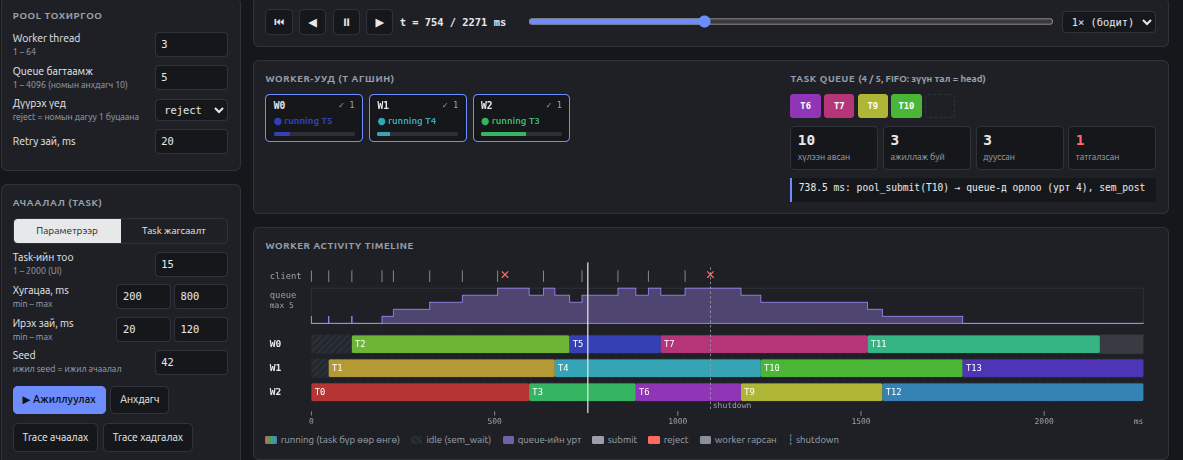
\includegraphics[width=0.88\linewidth]{img/user/ui_default_754.png}}}
\caption{Интерфейсийн ерөнхий харагдац: 3 worker, queue 5, 15 task-ийн бодит ажиллалт, t = 754 мс агшин (3 worker running, queue-д 4 task, 1 татгалзал)}\label{fig:overview}
\end{figure}

\subsection{GitHub дээрх ажиллагаа}

Repository: \url{https://github.com/NominjinNomio/F.CSM302-BD_IV-2-9-threadpool}. README (Quick Start), \code{src/}, \code{tests/}, \code{examples/}, \code{tools/}, \code{ui/}, \code{docs/} бүтэцтэй. \code{.github/workflows/ci.yml} нь push болон Pull Request бүрт Ubuntu дээр build, \code{make test}, ThreadSanitizer, macOS дээр clang build ба тестийг ажиллуулна. Гишүүн бүрийн хариуцсан хэсэг, commit-ийг Хавсралт А-д тэмдэглэв. 9-р долоо хоногт \code{v1.0} tag ба GitHub Release нийтэлнэ.

\subsection{Source}

Номын API-ийн нэр, \code{client.c} жишээний бүтцийг сурах бичгээс авсан. Код, интерфейс, тест, баримт бичгийн анхны хувилбарыг AI туслахын тусламжтайгаар бичиж, баг бүх өөрчлөлтийг бодит C программ дээр ажиллуулан тест болон гараар шалгасан. Гадны сан, бэлэн component ашиглаагүй. Дэлгэрэнгүйг README-ийн "AI ба бэлэн код ашигласан тухай" хэсгээс харна.

% ======================================================================
\section{Туршилт ба UI дүрслэл}

\subsection{Өөрчилж турших параметр}

\begin{longtable}{|P{0.220}|P{0.540}|P{0.240}|}
\caption{Тохиргооны параметр}\label{tab:params}\\
\hline
\rowcolor{tablehead} \textbf{Параметр} & \textbf{Нөлөө} & \textbf{Хүрээ (анхдагч)} \\ \hline
\endfirsthead
\hline
\rowcolor{tablehead} \textbf{Параметр} & \textbf{Нөлөө} & \textbf{Хүрээ (анхдагч)} \\ \hline
\endhead
Worker thread & зэрэг ажиллах thread-ийн тоо; timeline-ийн мөрийн тоо & 1-64 (3) \\ \hline
Queue багтаамж & хүлээж болох task-ийн тоо; бага бол татгалзал олширно & 1-4096 (5) \\ \hline
Дүүрэх үед & reject: номын дагуу 1 буцааж хаяна; retry: client хүлээгээд дахин оролдоно & reject \\ \hline
Retry зай (мс) & retry горимд дахин оролдох хоорондын зай & 1-10000 (20) \\ \hline
Task-ийн тоо & үүсгэх task-ийн тоо & 1-2000 (15) \\ \hline
Хугацаа (мс) & task бүрийн ажиллах хугацааны муж & 1-60000 (200-800) \\ \hline
Ирэх зай (мс) & дараалсан task-уудын хоорондох зай; 0 бол бүгд зэрэг & 0-60000 (20-120) \\ \hline
Seed & ижил seed = ижил ачаалал & ≥ 0 (42) \\ \hline
Task жагсаалт & мөр бүр \code{arrival\_ms duration\_ms}; бэлэн тест сонгож болно & ≤ 2000 мөр \\ \hline
\end{longtable}

\begin{figure}[H]
\centering
{\setlength{\fboxsep}{0pt}\setlength{\fboxrule}{0.5pt}\fcolorbox{frameline}{white}{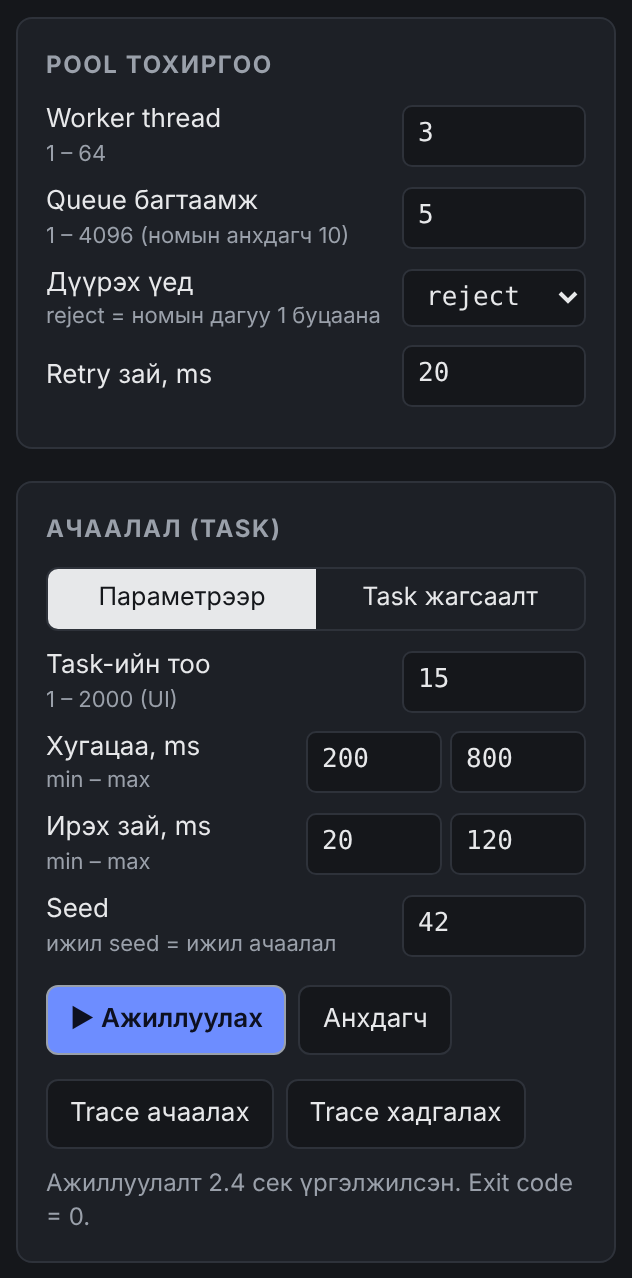
\includegraphics[width=0.38\linewidth]{img/shots/settings.png}}}
\caption{Тохиргоо: pool, ачаалал, ажиллуулах товч}\label{fig:settings}
\end{figure}

\subsection{Юуг ажиглах}

\begin{itemize}
  \item Queue хоосон үед worker-ууд "○ idle — sem\_wait" төлөвтэй, timeline дээр судалтай саарал байна; task ирмэгц нэг нь сэрж running болно.
  \item Worker бүх нь завгүй үед task-ууд queue-д хуримтлагдаж, queue-ийн уртын график өснө; task хамгийн зүүн (head) талаас нь авагдана (FIFO).
  \item Queue дүүрсэн үед client мөрөнд улаан ✕ гарч, "татгалзсан" тоолуур өснө (\code{pool\_submit} 1 буцаасан).
  \item Нэг worker нэг мөчид зөвхөн нэг task-тай; нэгэн зэрэг ажиллах task-ийн тоо worker-ийн тооноос хэтрэхгүй.
  \item Shutdown (тасархай зураас)-ы дараа queue-д үлдсэн task-ууд гүйцэтгэгдэж, дараа нь worker бүр гарна (бараан бүс).
\end{itemize}

\subsection{Бэлэн туршилтууд}

\begin{table}[H]
\centering
\caption{Интерфейсийн бэлэн туршилт}\label{tab:presets}
\begin{tabular}{|P{0.330}|P{0.300}|P{0.370}|}
\hline
\rowcolor{tablehead} \textbf{Туршилт} & \textbf{Тохиргоо} & \textbf{Хүлээгдсэн ажиглалт} \\ \hline
\code{basic.txt} & W=3, Q=10, 10 task & бүх task хүлээн авагдаж, зэрэг ≤ 3 \\ \hline
\code{burst.txt} & W=2, Q=3, 10 task t=0, reject & 3-5 хүлээн авч, үлдсэнийг татгалзана \\ \hline
\code{burst.txt} & W=2, Q=3, retry & 10 бүгд хүлээн авагдана, нийт хугацаа уртасна \\ \hline
\code{fifo.txt} & W=1, Q=10, 6 task & ирсэн дарааллаараа T0…T5 \\ \hline
\code{mixed\_long\_short.txt} & W=3, 1×1500 мс + 7×100 мс & урт task нэг worker-ийг эзэлж, бусад нь богинуудыг гүйцэтгэнэ \\ \hline
\end{tabular}
\end{table}

% ======================================================================
\section{Туршилтын арга}

\subsection{Орчин}

Хөгжүүлэлт ба автомат туршилт: Ubuntu 24.04.5 LTS (x86\_64, kernel 6.18.44-fc-v185), gcc 13.3.0, glibc 2.39, Python 3.13.18, CPU: Intel(R) Xeon(R) Processor @ 2.80GHz, 2 core. Интерфейсийг Chromium (headless) дээр туршиж дэлгэцийн зургийг авав. CI: GitHub Actions ubuntu-latest (gcc), macos-latest (clang). Windows дээр WSL2 Ubuntu-аар ажиллана.

Үүнээс гадна багийн гишүүн Ц.Номинжингийн Ubuntu компьютер дээр Manual-ын дагуу repository-г татаж, VS Code-ийн терминал болон дотоод browser-оос бүх командыг дахин ажиллуулж шалгав (8.4 хэсэг).

\subsection{Core-ийн автомат тест}

\code{tests/run\_tests.sh} нь программыг олон тохиргоогоор ажиллуулж, гарсан trace-ийг шалгана:

\begin{itemize}
  \item \textbf{Номын жишээ (T1)}: \code{examples/client.c} 5 нийлбэрийг зөв хэвлэх.
  \item \textbf{Үндсэн (T2-T7)}: анхдагч тохиргоо, queue дүүрэх (reject, retry), FIFO, урт ба богино task, санамсаргүй ачаалал.
  \item \textbf{Захын (B1-B5)}: queue=1, worker > task, 64 worker, 1 task, 500 task-ийн stress.
  \item \textbf{Буруу оролт (E1-E17)}: 0 ба 65 worker, queue=0, тоо биш утга, MIN > MAX, сөрөг зай, үл мэдэгдэх бодлого/сонголт, утгагүй сонголт, байхгүй файл, файлд тоо биш утга, эрэмбэгүй мөр, 3 баганатай мөр, 0 хугацаа, хоосон файл. Exit код 2 ба алдааны текстийг шалгана.
\end{itemize}

\subsection{Trace шалгагч ба ThreadSanitizer}

\code{tests/verify\_trace.py} нь C кодоос хараат бусаар: queue-ийн уртыг SUBMIT/START-аас дахин сэргээж бүртгэсэн \code{q}-тэй тулгах; нэг worker дээрх интервал давхцахгүй; START-ийн дараалал = SUBMIT-ийн дараалал (FIFO); SHUTDOWN-ы дараа SUBMIT байхгүй; worker бүр WORKER\_EXIT хийсэн эсэхийг шалгана. Мөн тест бүрт хүлээгдсэн тоог (\code{--expect accepted=10} гэх мэт) тулгана. \code{make tsan} нь \code{-fsanitize=thread}-тэй build хийж, 4 worker, queue 3, 40 task, retry горимоор өрсөлдөөнийг ихэсгэн ажиллуулна.

\subsection{Гүйцэтгэлийн туршилт}

\code{tests/experiments.sh} нь worker-ийн тоо, queue-ийн багтаамж, дүүрэх үеийн бодлогыг тус тусад нь өөрчилж, бусад параметрийг тогтмол барина (seed тогтмол).

\subsection{Гар туршилт}

Интерфейсийн бэлэн туршилтууд, буруу оролт (worker 0, task жагсаалтад тоо биш утга), алхамчлах, хурд солих, trace хадгалах ба сервергүйгээр ачаалахыг browser дээр гараар туршиж, дэлгэцийн зургаар баримтжуулав (8-р бүлэг).

% ======================================================================
\section{Үр дүн}

\subsection{Core-ийн тестийн үр дүн}

Linux дээрх ажиллалтын үр дүн (Хүснэгт \ref{tab:tests}). Бодит үр дүн баганын тоо \code{build/test\_output.txt}-ээс шууд авсан.

\begin{longtable}{|P{0.100}|P{0.340}|P{0.460}|P{0.100}|}
\caption{Автомат тестийн үр дүн (\code{make test}, \code{make tsan})}\label{tab:tests}\\
\hline
\rowcolor{tablehead} \textbf{ID} & \textbf{Тест} & \textbf{Бодит үр дүн} & \textbf{Дүн} \\ \hline
\endfirsthead
\hline
\rowcolor{tablehead} \textbf{ID} & \textbf{Тест} & \textbf{Бодит үр дүн} & \textbf{Дүн} \\ \hline
\endhead
T1 & Номын \code{client.c} & 15, 3, 300, 0, 42 зөв хэвлэгдсэн & PASS \\ \hline
T2 & Номын анхдагч 3 worker, queue 10, 10 task & хүлээн авсан 10, татгалзсан 0, зэрэг 3, queue 4 & PASS \\ \hline
T3 & Burst: 10 task t=0, 2 worker, queue 3, reject & хүлээн авсан 3, татгалзсан 7, зэрэг 2, queue 3 & PASS \\ \hline
T4 & Burst, retry горим & хүлээн авсан 10, татгалзсан 0, зэрэг 2, queue 3 & PASS \\ \hline
T5 & 1 worker: FIFO дараалал & хүлээн авсан 6, татгалзсан 0, зэрэг 1, queue 5 & PASS \\ \hline
T6 & 1 урт + 7 богино task, 3 worker & хүлээн авсан 8, татгалзсан 0, зэрэг 3, queue 5 & PASS \\ \hline
T7 & 4 worker, queue 8, 20 санамсаргүй task & хүлээн авсан 20, татгалзсан 0, зэрэг 4, queue 5 & PASS \\ \hline
B1 & queue=1, 1 worker, 6 task зэрэг & хүлээн авсан 1, татгалзсан 5, зэрэг 1, queue 1 & PASS \\ \hline
B2 & 8 worker, 3 task (worker > task) & хүлээн авсан 3, татгалзсан 0, зэрэг 3, queue 3 & PASS \\ \hline
B3 & 64 worker (дээд хязгаар), 64 task & хүлээн авсан 64, татгалзсан 0, зэрэг 64, queue 27 & PASS \\ \hline
B4 & 1 task, 1 мс & хүлээн авсан 1, татгалзсан 0, зэрэг 1, queue 1 & PASS \\ \hline
B5 & 500 task, 8 worker, queue 16, retry & хүлээн авсан 500, татгалзсан 0, зэрэг 8, queue 16 & PASS \\ \hline
E1-E17 & Буруу оролт & exit=2, тохирох тайлбар (жишээ нь "-w буруу ('0'): worker-ийн тоо 1..64 бүхэл тоо байна") & PASS \\ \hline
R1 & ThreadSanitizer & race илрээгүй, VERIFY: OK & PASS \\ \hline
\end{longtable}

Нийт 29/29 PASS. Бүх тестийн trace хараат бус шалгагчаар баталгаажсан, ThreadSanitizer race илрүүлээгүй. B3 тестэд 64 worker бүгд зэрэг ажилласан, B5 тестэд 500 task бүр яг 1 удаа гүйцэтгэгдсэн.

\subsection{Гүйцэтгэлийн туршилтын үр дүн}

\textbf{Туршилт 1. Worker-ийн тоо.} 40 task, хугацаа 100-300 мс, бүгд t=0-д ирнэ, queue 64, seed 1.

\begin{table}[H]
\centering
\caption{Worker-ийн тооны нөлөө}\label{tab:exp1}
\begin{tabular}{|P{0.167}|P{0.167}|P{0.167}|P{0.167}|P{0.167}|P{0.167}|}
\hline
\rowcolor{tablehead} \textbf{Worker} & \textbf{Нийт хугацаа (мс)} & \textbf{Дундаж хүлээлт (мс)} & \textbf{Дундаж turnaround (мс)} & \textbf{Ашиглалт (\%)} & \textbf{Хурдатгал} \\ \hline
1 & 8377 & 4021 & 4230 & 100.0 & 1.00× \\ \hline
2 & 4223 & 1955 & 2164 & 99.2 & 1.98× \\ \hline
4 & 2196 & 921 & 1131 & 95.3 & 3.81× \\ \hline
8 & 1139 & 406 & 616 & 91.9 & 7.35× \\ \hline
16 & 647 & 151 & 360 & 81.0 & 12.96× \\ \hline
\end{tabular}
\end{table}

Нийт хугацаа worker-ийн тоонд бараг урвуу пропорциональ буурсан (2 worker → 1.98×, 8 worker → 7.35×). 16 worker-т ашиглалт 81\% хүртэл буурсан: 40 task 16 worker-т тэгш хуваагдахгүй тул сүүлийн давалгаанд зарим worker idle үлдэнэ.

\textbf{Туршилт 2. Queue-ийн багтаамж.} 2 worker, 20 task t=0-д, тус бүр 100 мс, reject.

\begin{table}[H]
\centering
\caption{Queue-ийн багтаамжийн нөлөө}\label{tab:exp2}
\begin{tabular}{|P{0.200}|P{0.200}|P{0.200}|P{0.200}|P{0.200}|}
\hline
\rowcolor{tablehead} \textbf{Queue} & \textbf{Хүлээн авсан} & \textbf{Татгалзсан} & \textbf{Queue дээд урт} & \textbf{Нийт хугацаа (мс)} \\ \hline
1 & 1 & 19 & 1 & 100 \\ \hline
2 & 2 & 18 & 2 & 100 \\ \hline
4 & 4 & 16 & 4 & 201 \\ \hline
8 & 8 & 12 & 8 & 401 \\ \hline
16 & 16 & 4 & 16 & 802 \\ \hline
20 & 20 & 0 & 20 & 1002 \\ \hline
\end{tabular}
\end{table}

Хүлээн авсан task-ийн тоо багтаамжтай яг тэнцүү гарсан. Client 20 task-ийг микросекундын дотор submit хийдэг бол worker \code{sem\_wait}-аас сэрж dequeue хийхэд түүнээс урт хугацаа шаардана; иймээс burst-ийн үед queue хоосрохоос өмнө дүүрнэ.

\textbf{Туршилт 3. Дүүрэх үеийн бодлого.} 2 worker, queue 3, 20 task 10 мс зайтай, тус бүр 100 мс.

\begin{table}[H]
\centering
\caption{Reject ба retry бодлого}\label{tab:exp3}
\begin{tabular}{|P{0.200}|P{0.200}|P{0.200}|P{0.200}|P{0.200}|}
\hline
\rowcolor{tablehead} \textbf{Бодлого} & \textbf{Хүлээн авсан task} & \textbf{Татгалзсан оролдлого} & \textbf{Нийт хугацаа (мс)} & \textbf{Дундаж хүлээлт (мс)} \\ \hline
reject & 7 & 13 & 401 & 89 \\ \hline
retry & 20 & 38 & 1012 & 120 \\ \hline
\end{tabular}
\end{table}

Reject горимд task алдагдсан ч нийт хугацаа богино; retry горимд бүх task гүйцэтгэгдсэн боловч client хүлээсэн тул уртассан.

\subsection{Интерфейсийн үр дүн}

Зураг \ref{fig:burst}-\ref{fig:err} нь бодит программын ажиллалтаас авсан дэлгэцийн зураг.

\begin{figure}[H]
\centering
{\setlength{\fboxsep}{0pt}\setlength{\fboxrule}{0.5pt}\fcolorbox{frameline}{white}{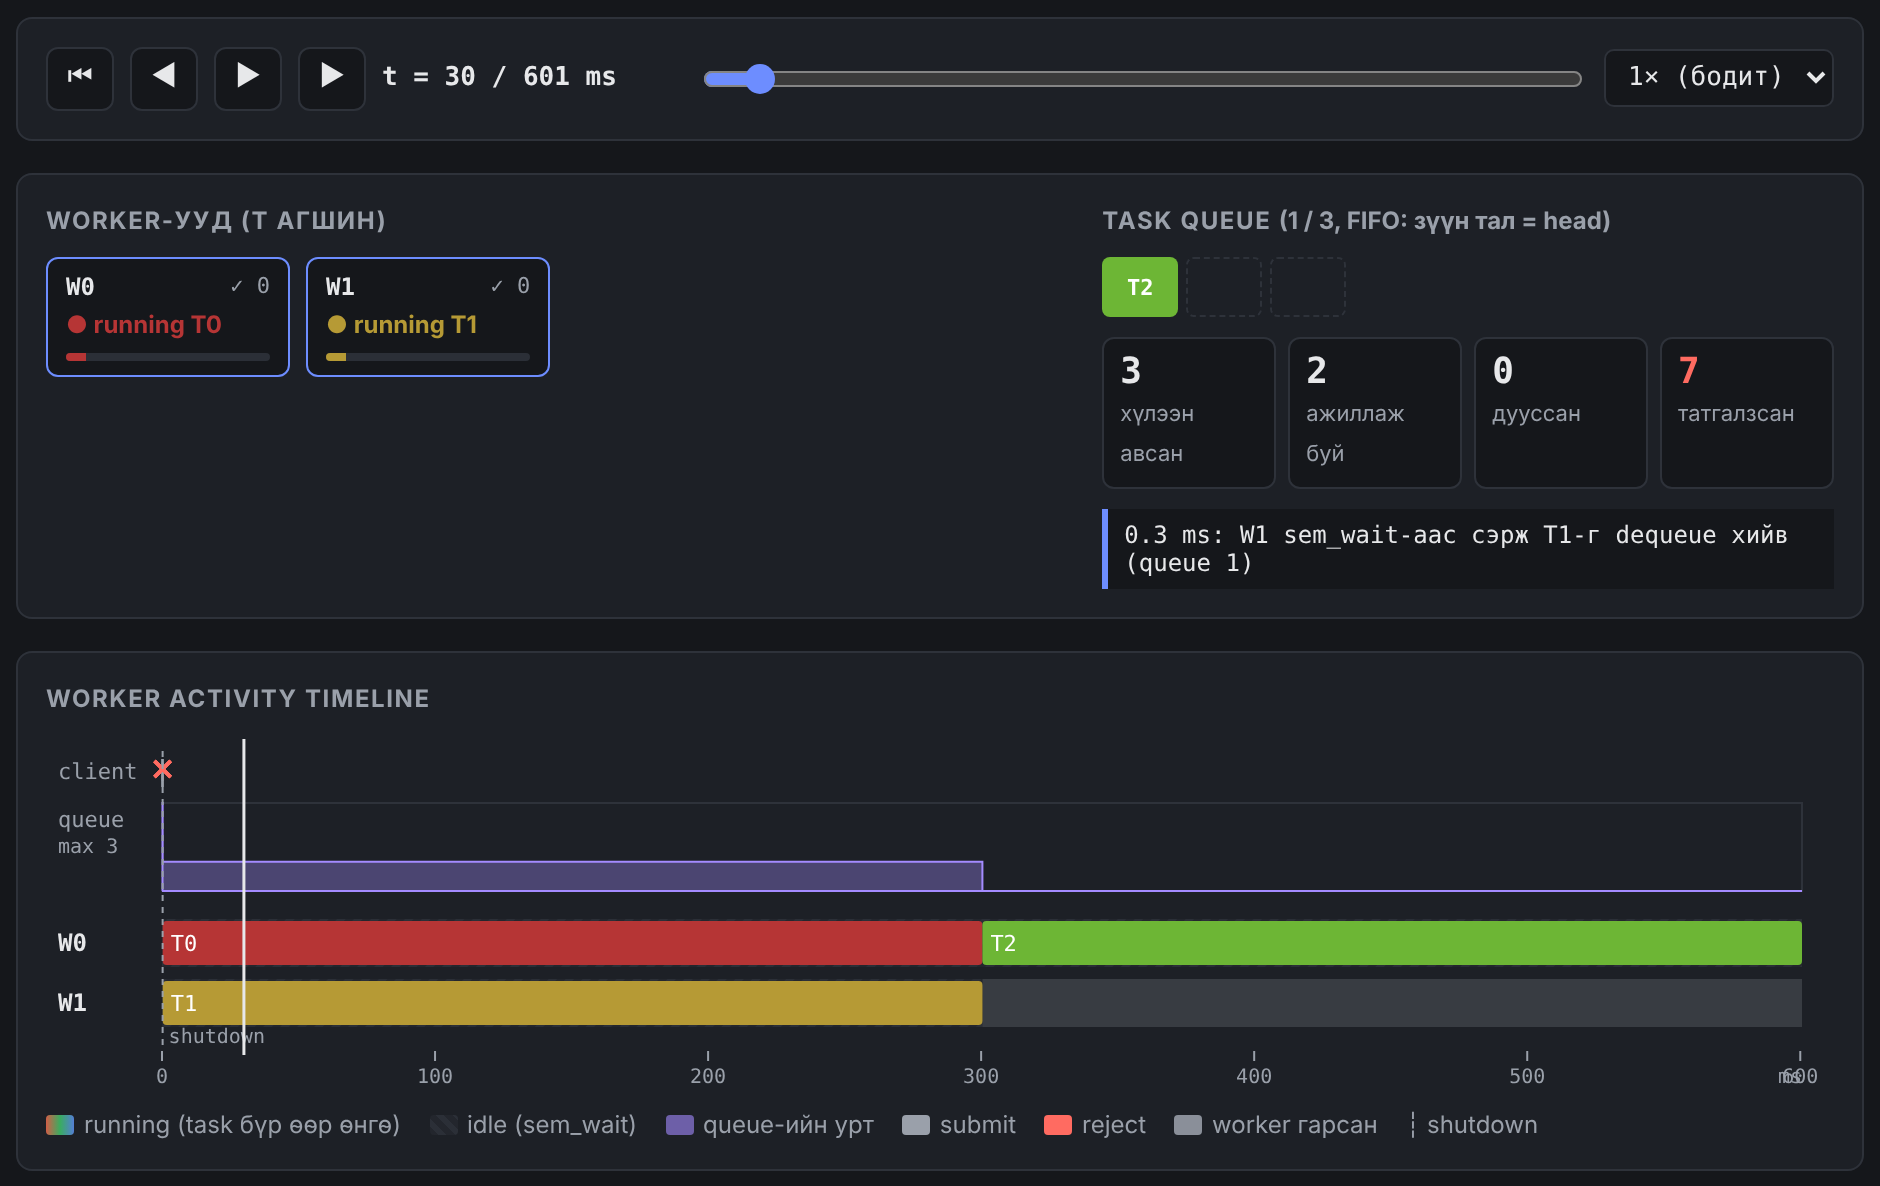
\includegraphics[width=0.72\linewidth]{img/shots/burst_reject.png}}}
\caption{Queue дүүрэх (W=2, Q=3, reject): t=30 мс-д T0, T1 ажиллаж, T2 queue-д, 7 task татгалзсан (client мөрөнд ✕)}\label{fig:burst}
\end{figure}

\begin{figure}[H]
\centering
{\setlength{\fboxsep}{0pt}\setlength{\fboxrule}{0.5pt}\fcolorbox{frameline}{white}{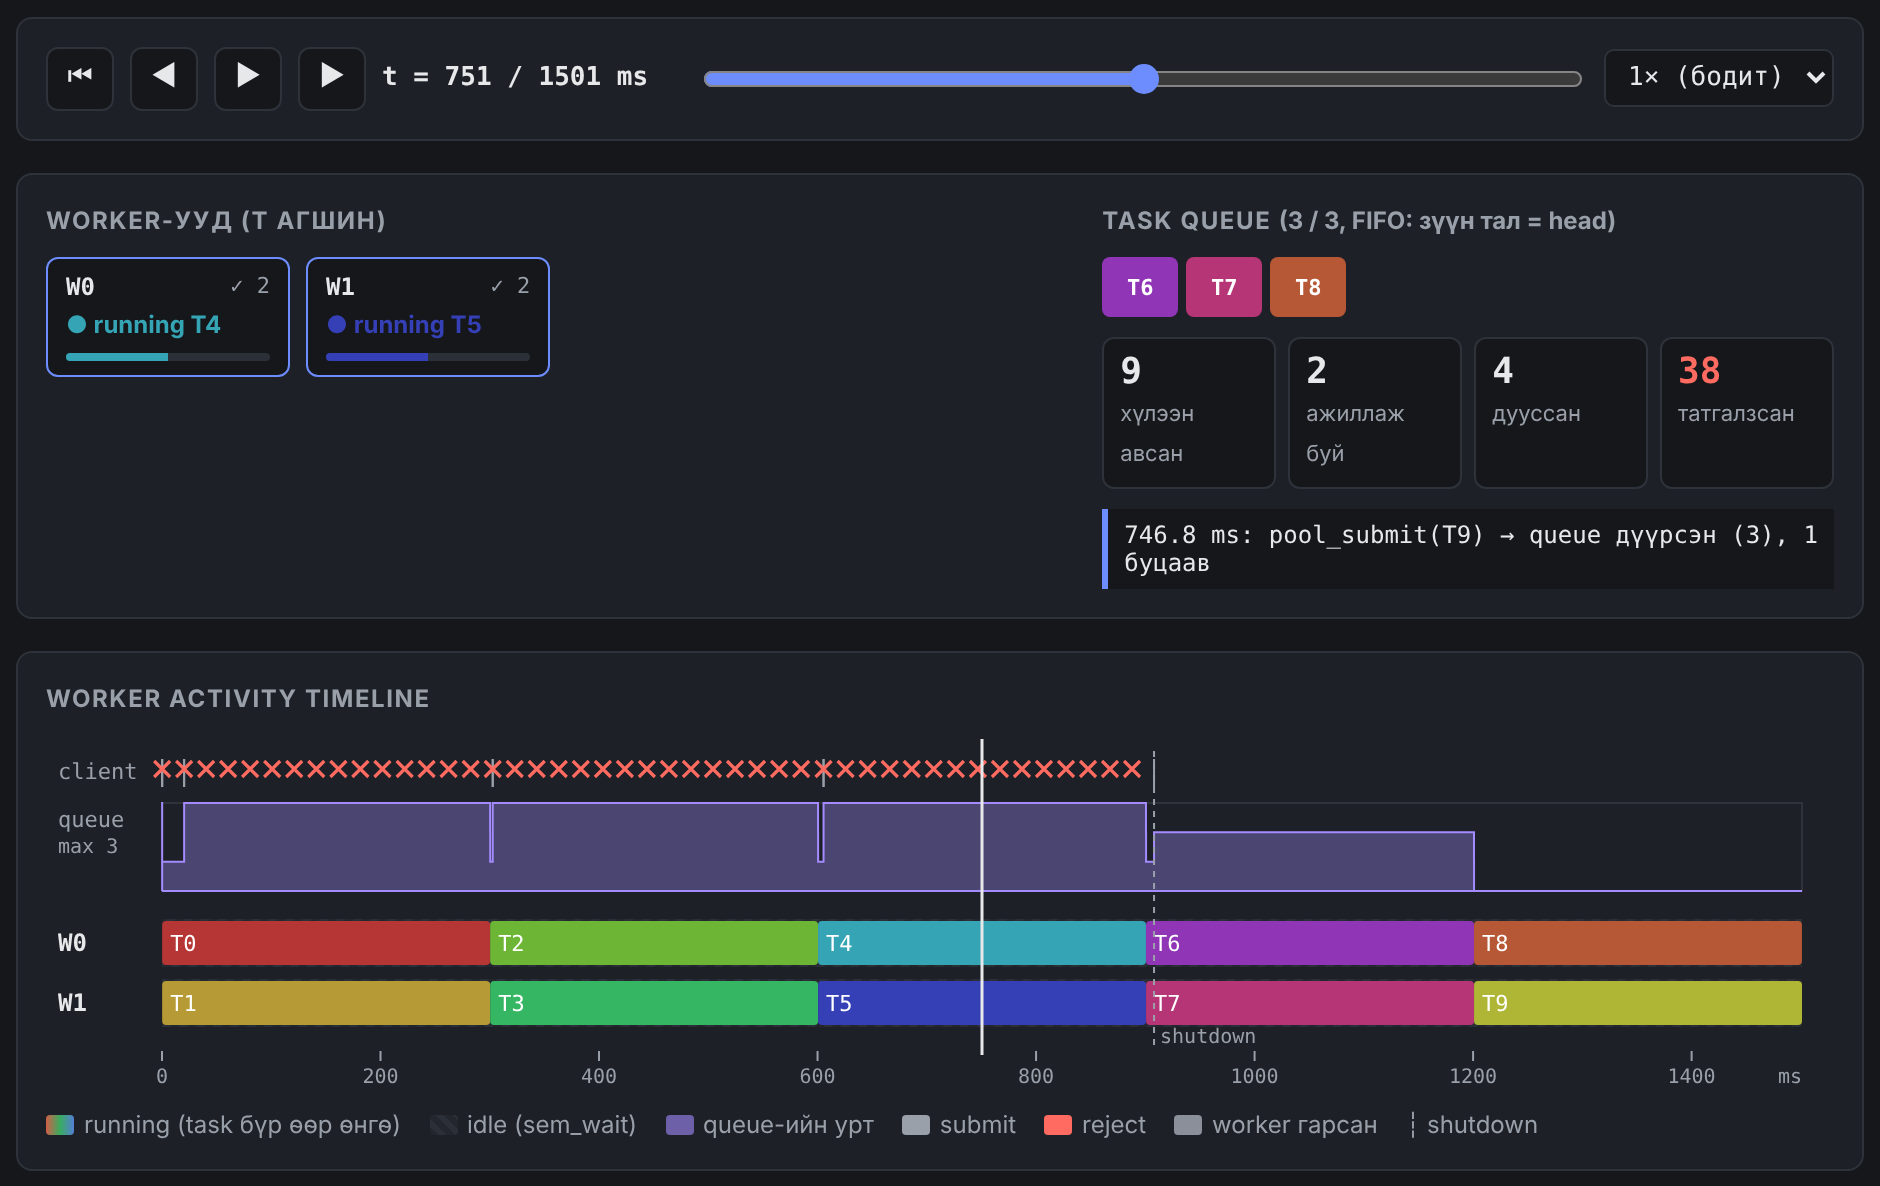
\includegraphics[width=0.72\linewidth]{img/shots/burst_retry.png}}}
\caption{Ижил ачаалал, retry горим: client дахин оролдож (✕ олон), 10 task бүгд гүйцэтгэгдсэн}
\end{figure}

\begin{figure}[H]
\centering
{\setlength{\fboxsep}{0pt}\setlength{\fboxrule}{0.5pt}\fcolorbox{frameline}{white}{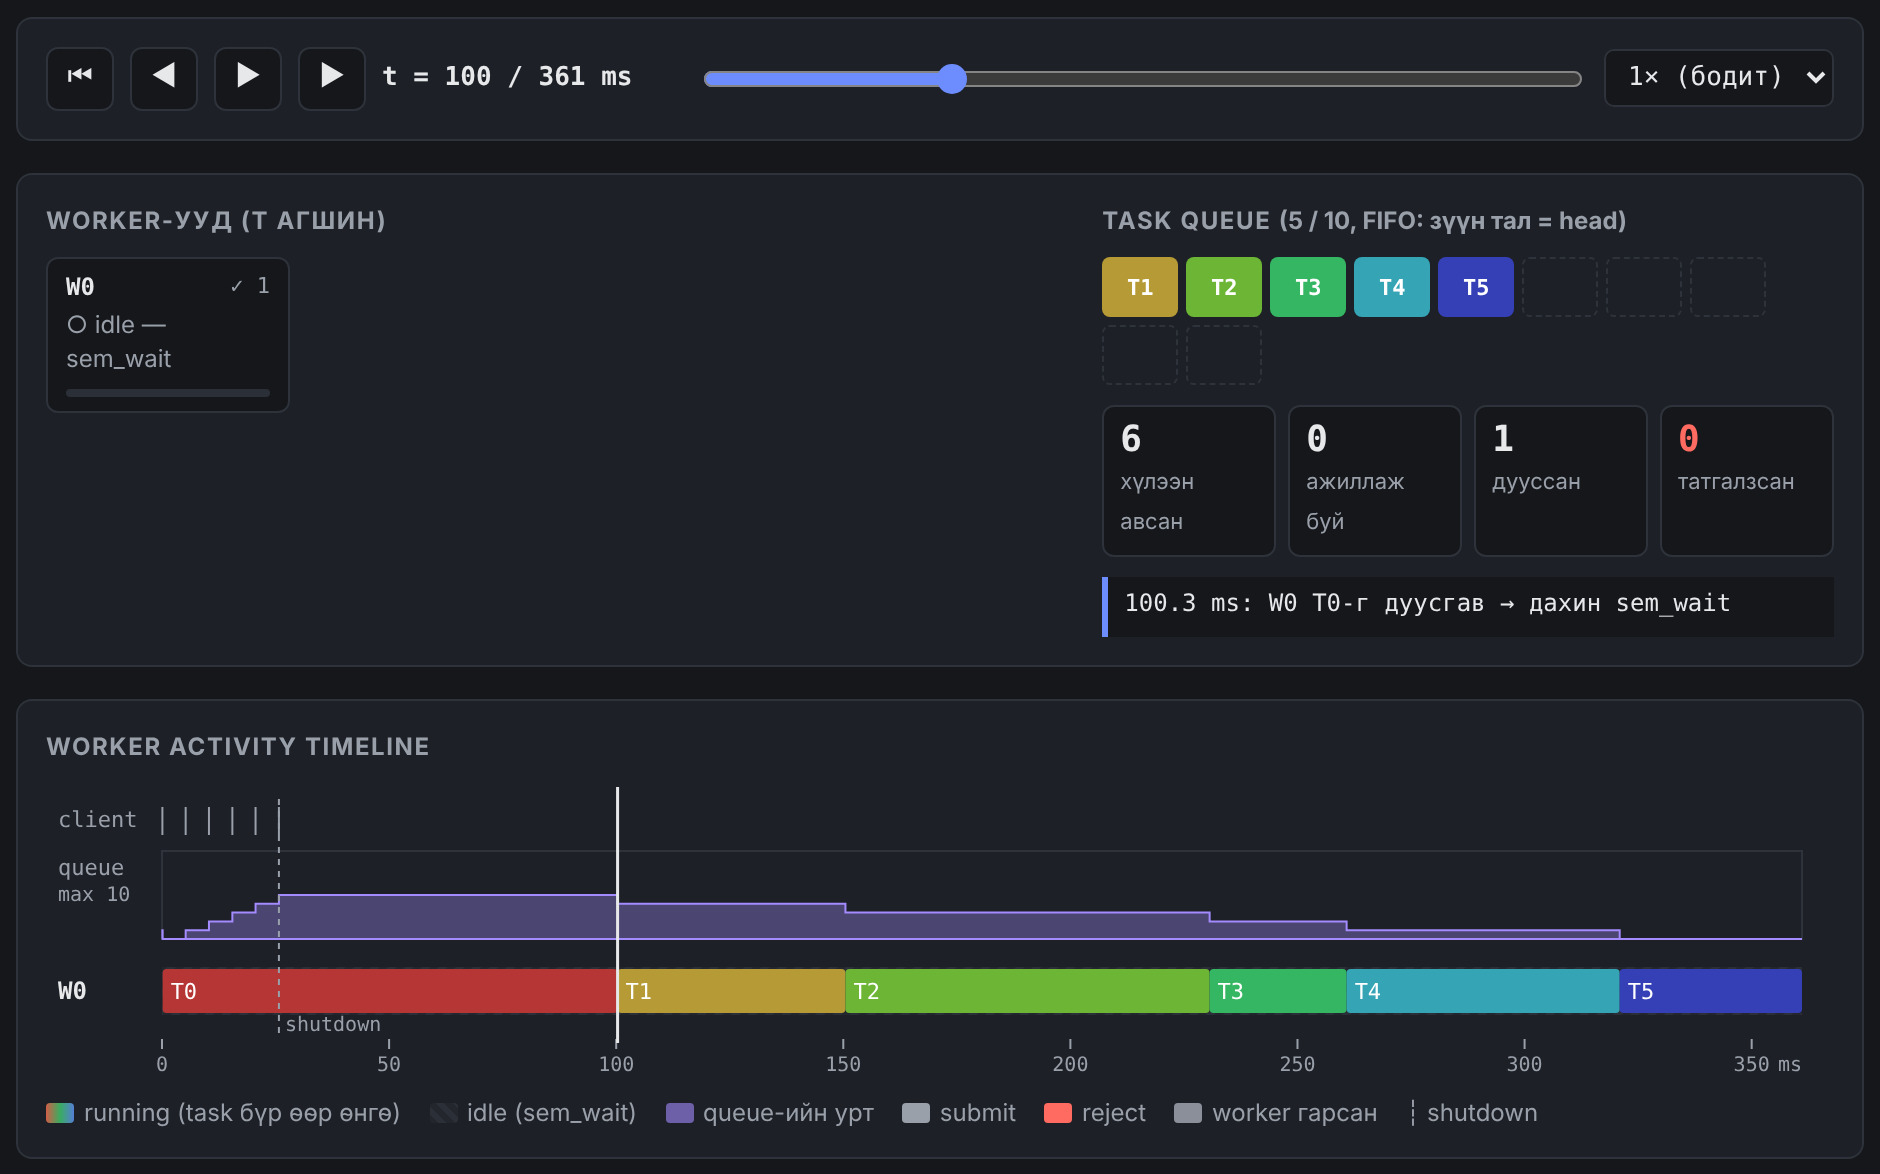
\includegraphics[width=0.72\linewidth]{img/shots/fifo_step.png}}}
\caption{FIFO (W=1): дараагийн үйлдэл товчоор алхамчилсан; T3, T4, T5 ирсэн дарааллаараа queue-д хүлээж байна}
\end{figure}

\begin{figure}[H]
\centering
{\setlength{\fboxsep}{0pt}\setlength{\fboxrule}{0.5pt}\fcolorbox{frameline}{white}{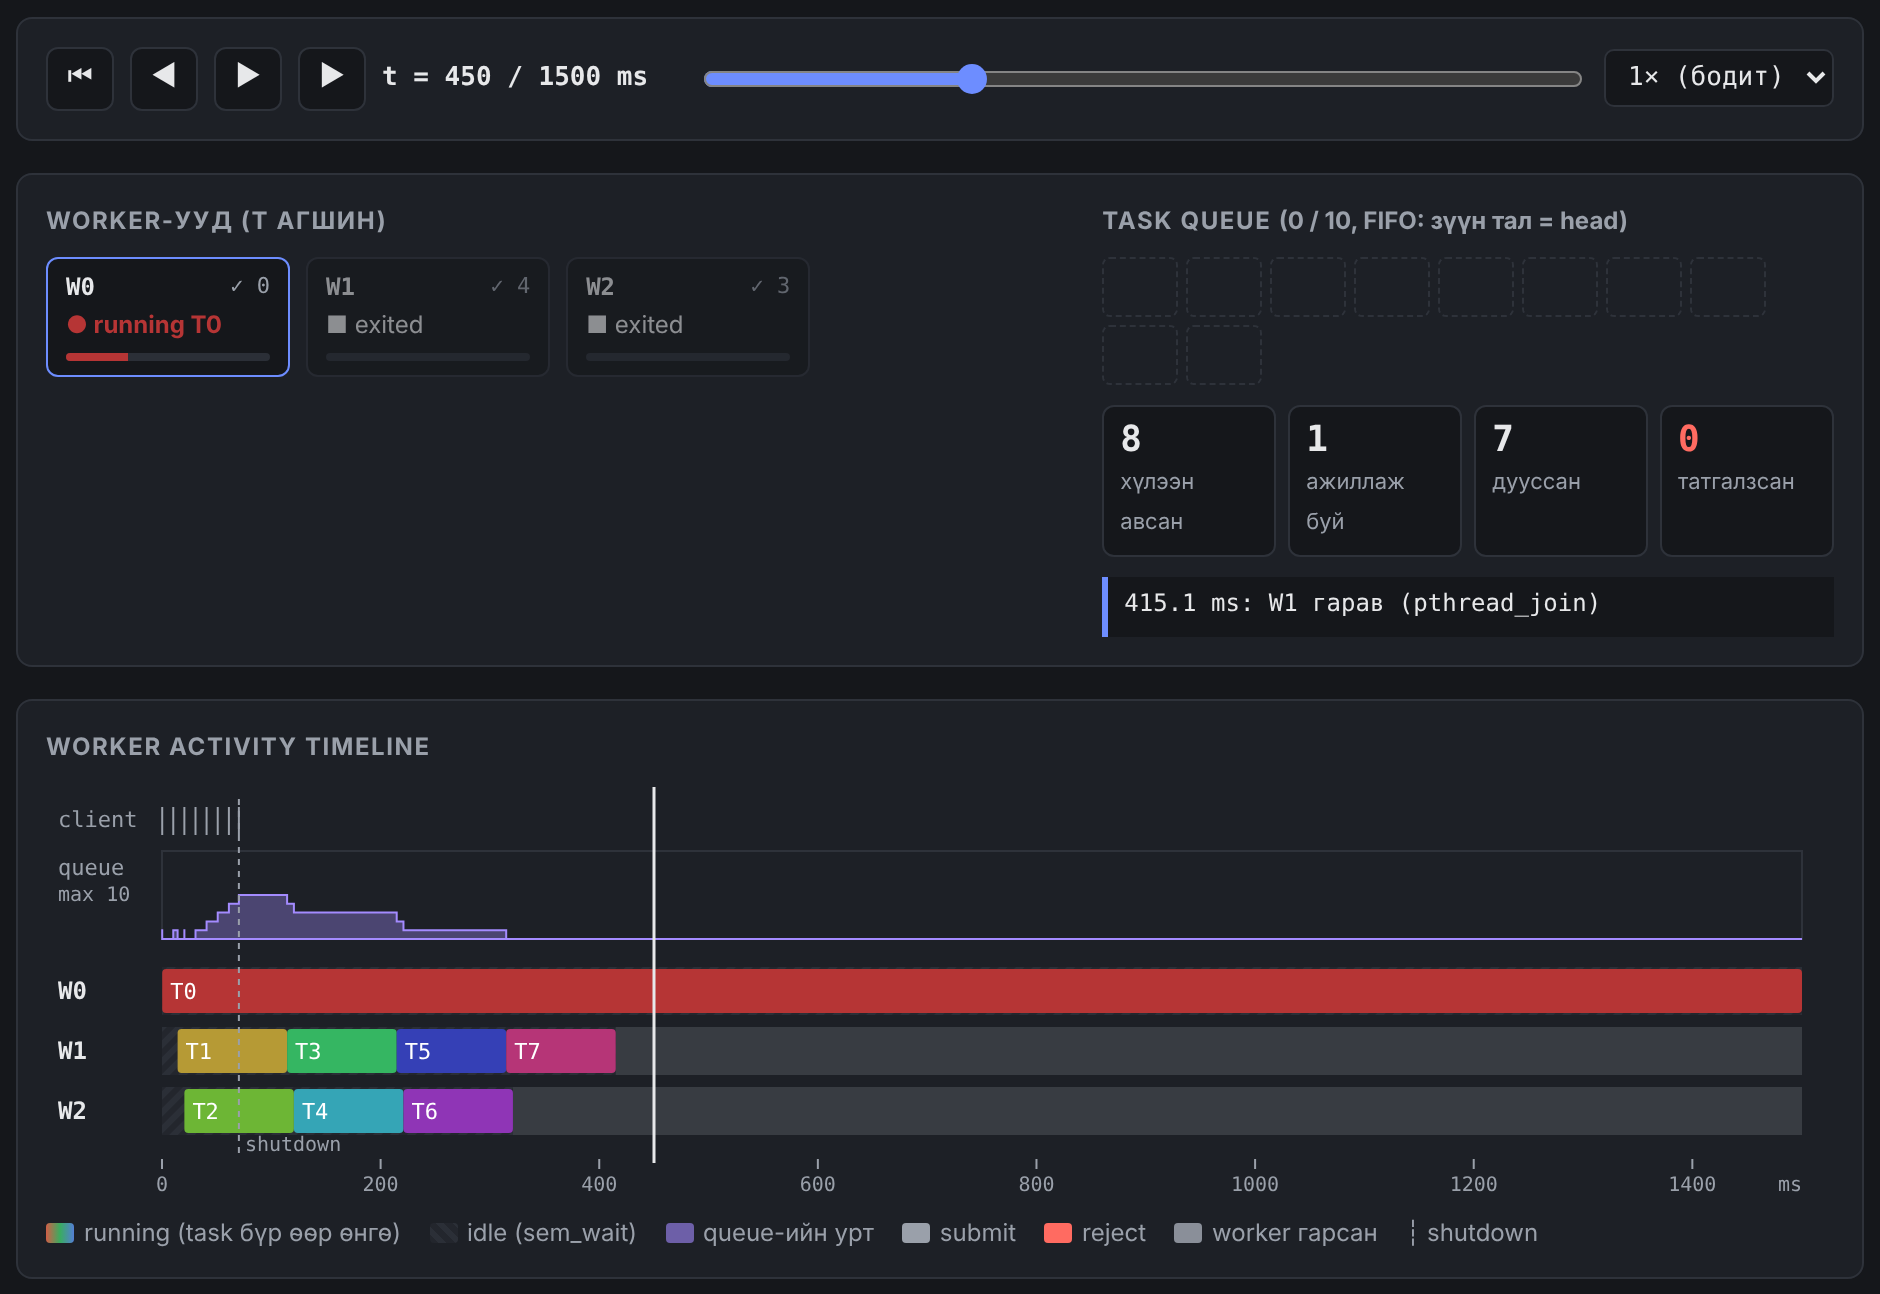
\includegraphics[width=0.72\linewidth]{img/shots/long_short.png}}}
\caption{Урт (T0 = 1500 мс) ба богино task: W0 урт task-аар эзлэгдсэн ч W1, W2 богинуудыг гүйцэтгэсээр}
\end{figure}

\begin{figure}[H]
\centering
{\setlength{\fboxsep}{0pt}\setlength{\fboxrule}{0.5pt}\fcolorbox{frameline}{white}{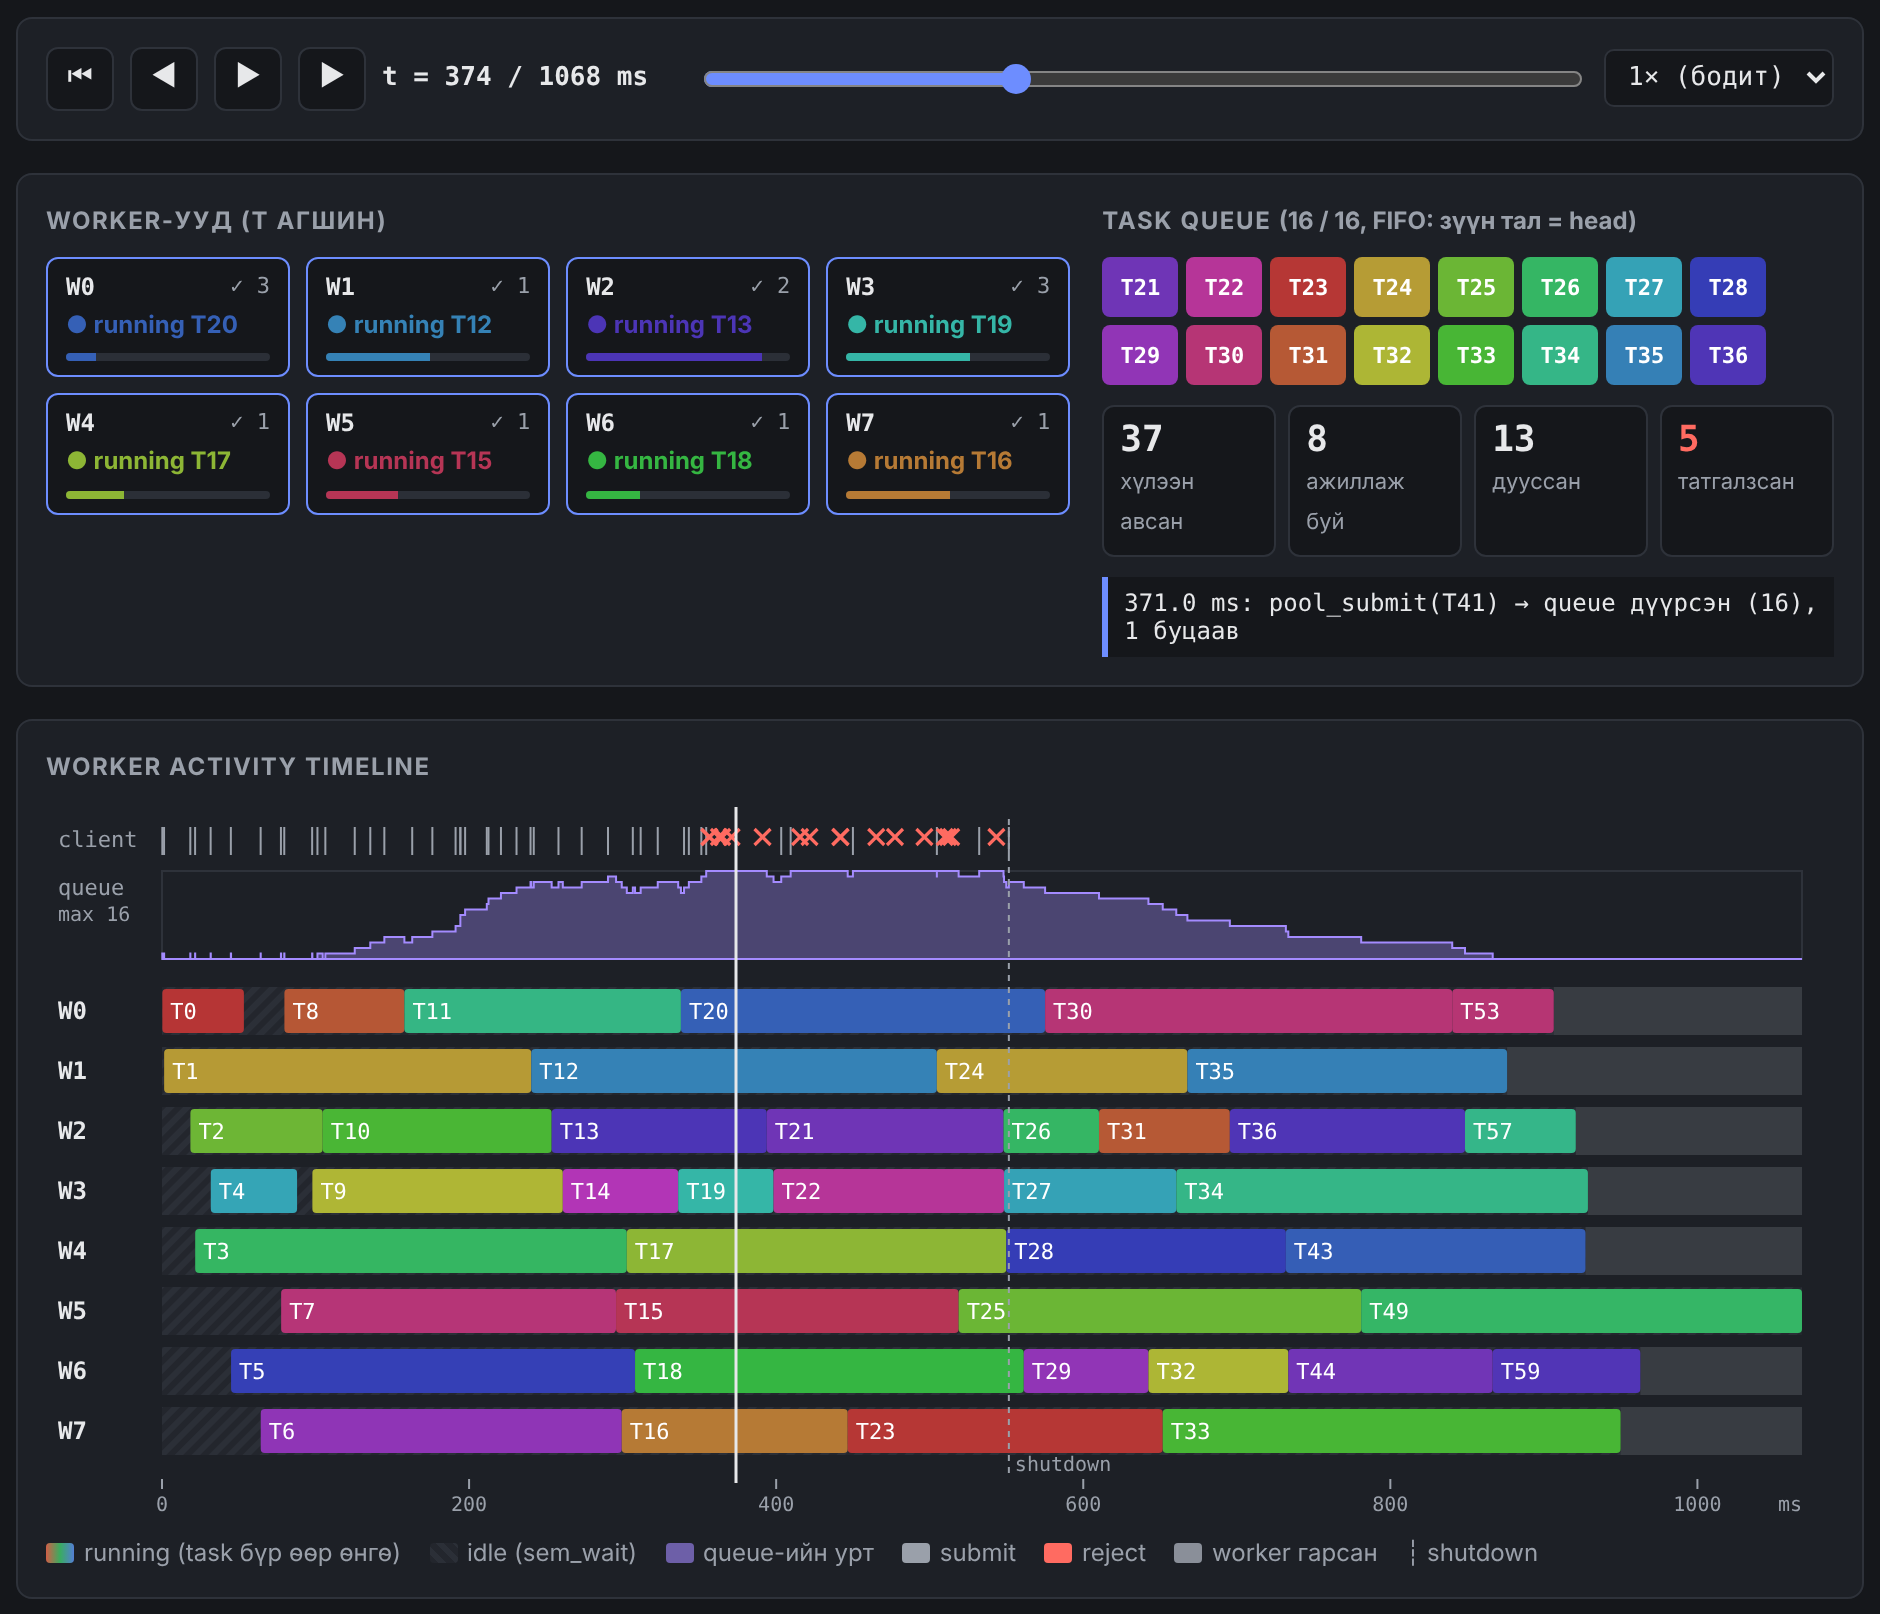
\includegraphics[width=0.72\linewidth]{img/shots/eight_workers.png}}}
\caption{8 worker, queue 16, 60 task: queue-ийн урт ачааллын давалгааг дагаж өсөж буурна}
\end{figure}

\begin{figure}[H]
\centering
{\setlength{\fboxsep}{0pt}\setlength{\fboxrule}{0.5pt}\fcolorbox{frameline}{white}{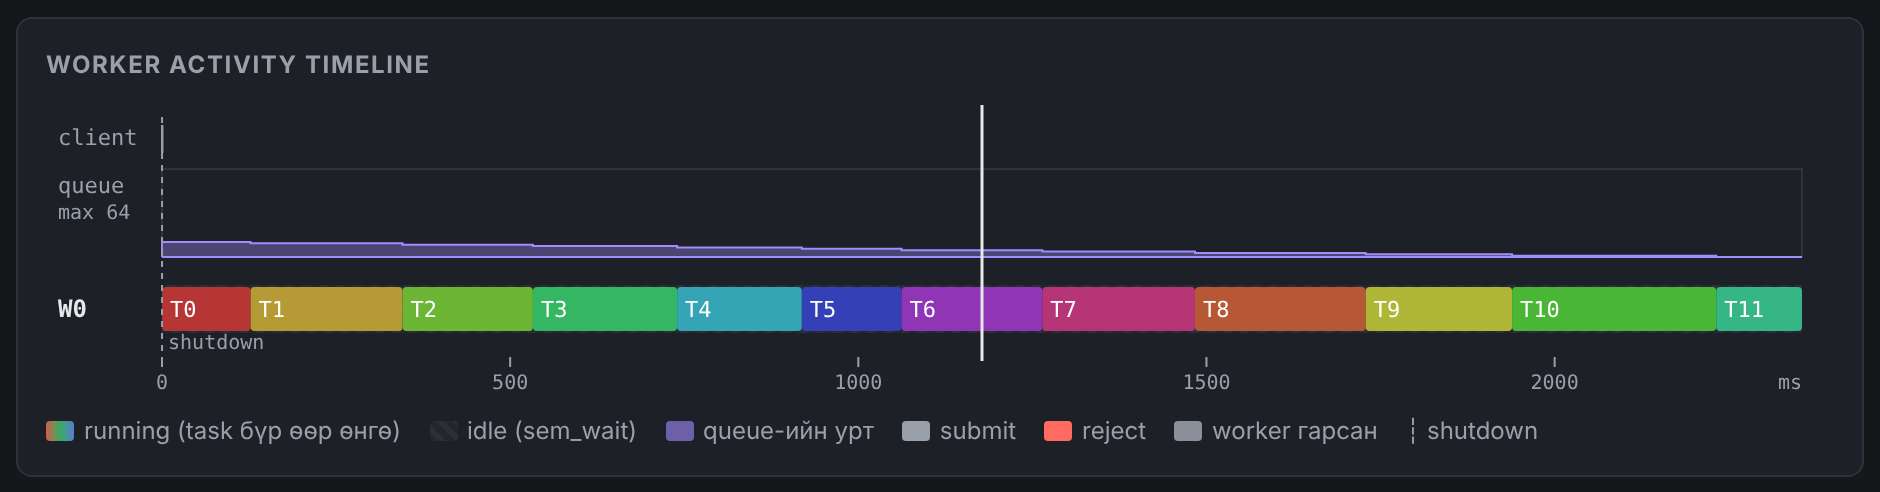
\includegraphics[width=0.78\linewidth]{img/shots/compare_w1.png}}}\\[8pt]
{\setlength{\fboxsep}{0pt}\setlength{\fboxrule}{0.5pt}\fcolorbox{frameline}{white}{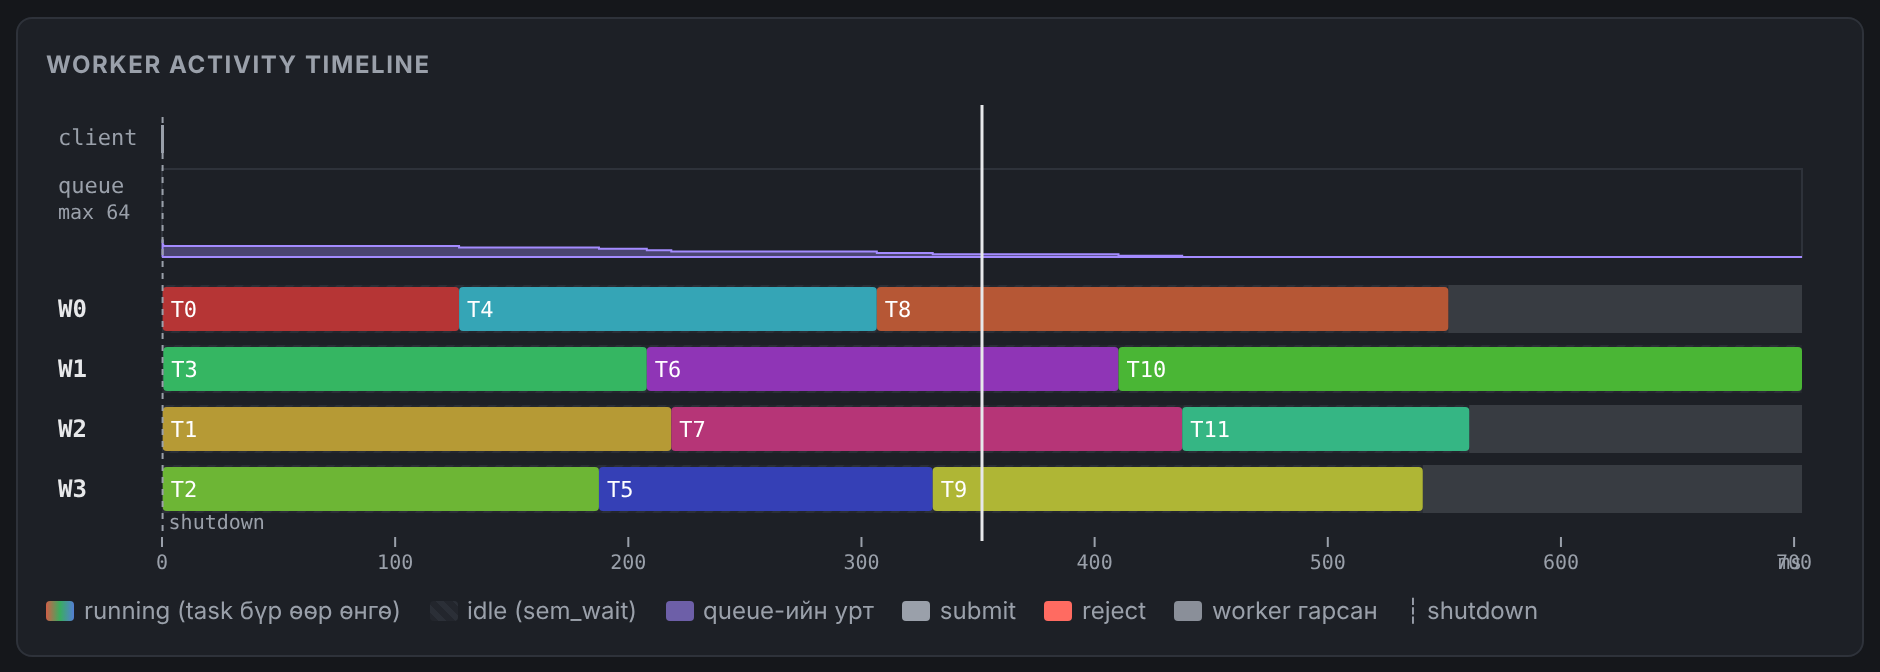
\includegraphics[width=0.78\linewidth]{img/shots/compare_w4.png}}}
\caption{Ижил 12 task (100-300 мс, seed 1): дээр 1 worker, доор 4 worker; нийт хугацаа ойролцоогоор 4 дахин богиносов}
\end{figure}

\begin{figure}[H]
\centering
{\setlength{\fboxsep}{0pt}\setlength{\fboxrule}{0.5pt}\fcolorbox{frameline}{white}{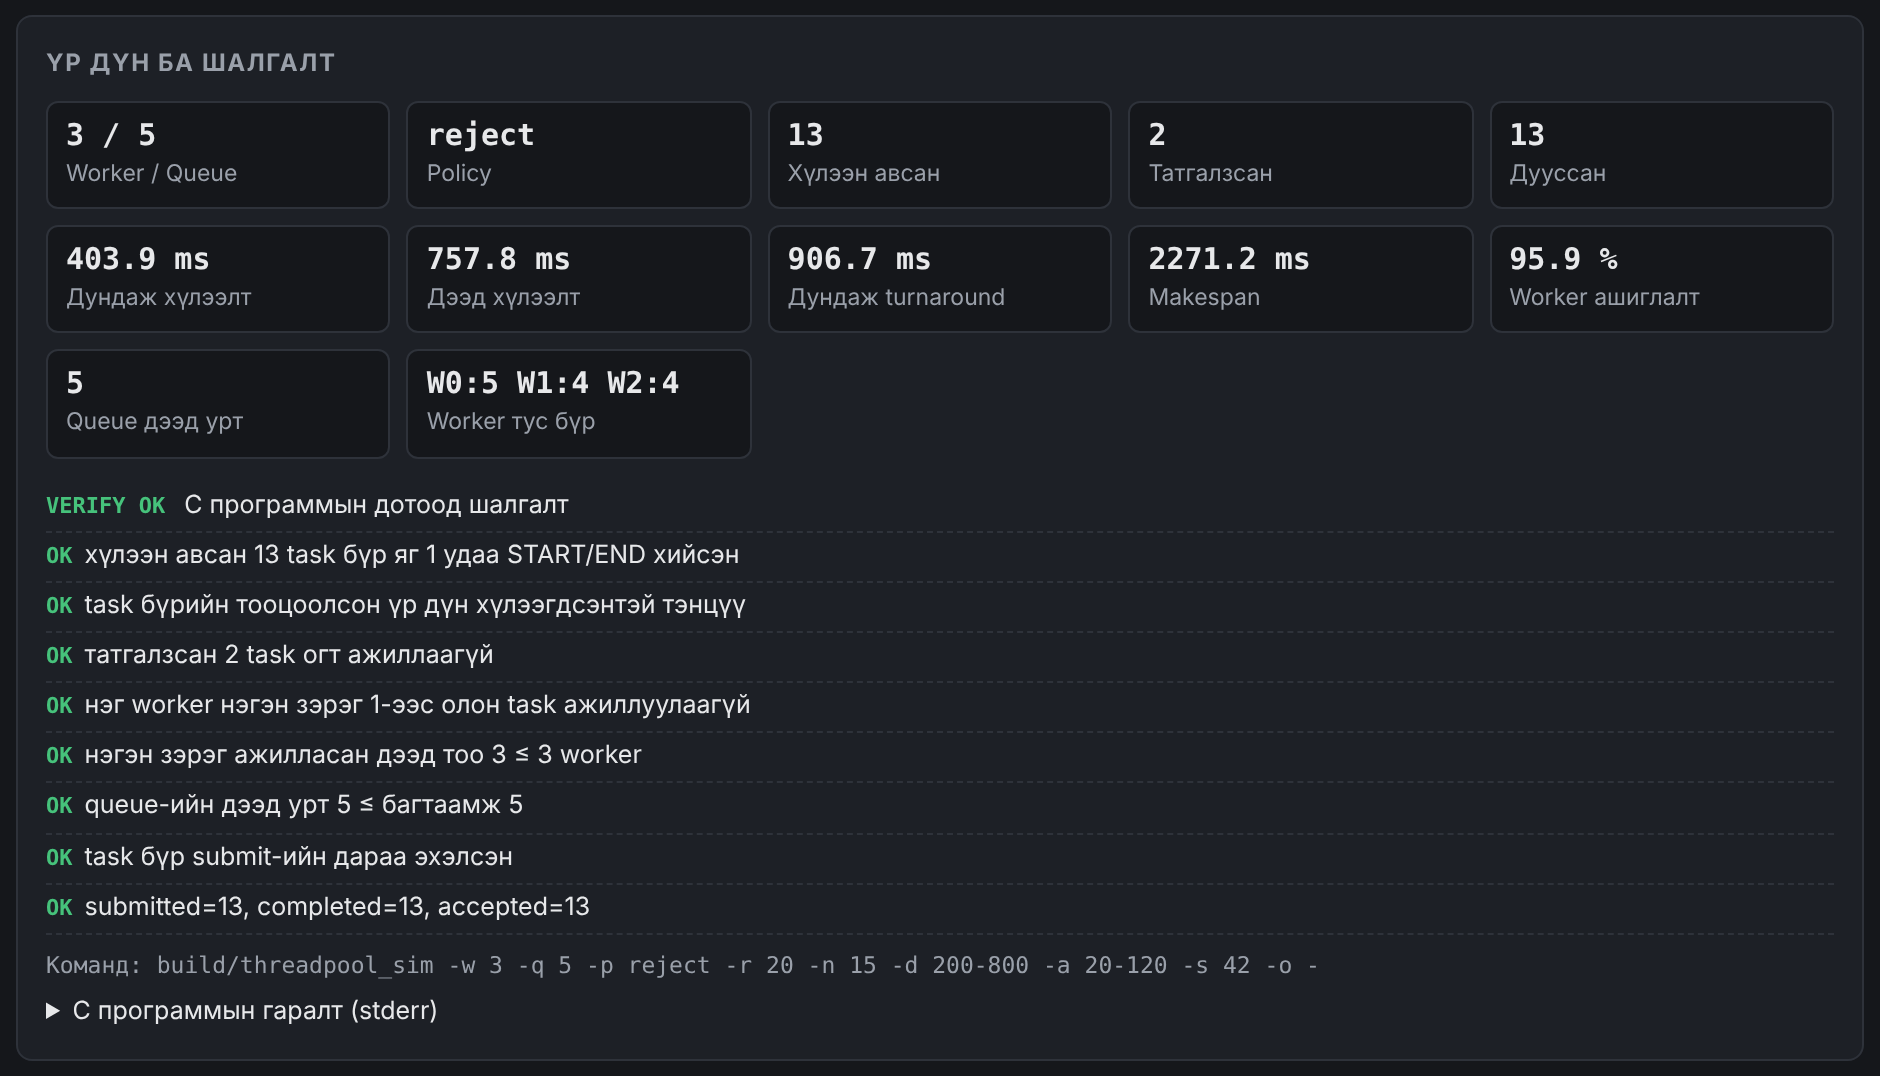
\includegraphics[width=0.72\linewidth]{img/shots/summary.png}}}
\caption{Үр дүн ба шалгалт: хэмжүүрүүд, VERIFY OK ба 8 шалгалт, C программын команд}\label{fig:summary}
\end{figure}

\begin{figure}[H]
\centering
\begin{minipage}[t]{0.384\linewidth}\vspace{0pt}{\setlength{\fboxsep}{0pt}\setlength{\fboxrule}{0.5pt}\fcolorbox{frameline}{white}{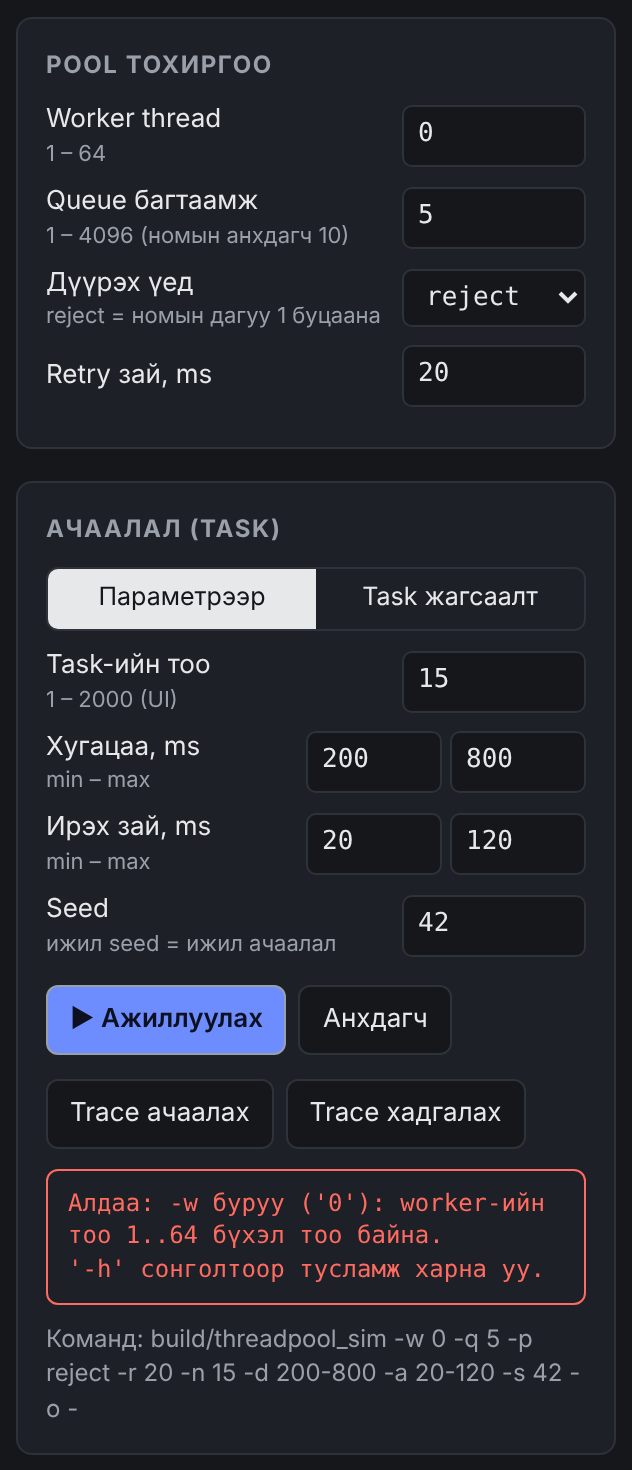
\includegraphics[width=\linewidth]{img/shots/error_workers0.png}}}\end{minipage}\hspace{4mm}\begin{minipage}[t]{0.384\linewidth}\vspace{0pt}{\setlength{\fboxsep}{0pt}\setlength{\fboxrule}{0.5pt}\fcolorbox{frameline}{white}{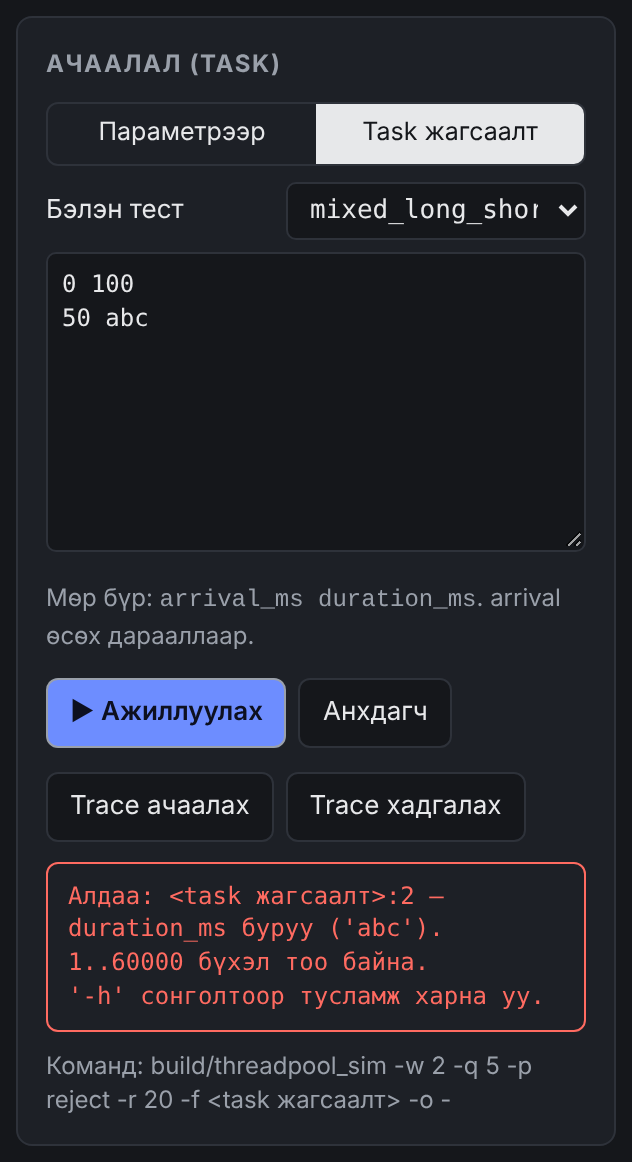
\includegraphics[width=\linewidth]{img/shots/error_file.png}}}\end{minipage}
\caption{Буруу оролт: зүүн талд worker = 0, баруун талд task жагсаалтын 2-р мөрөнд тоо биш утга}\label{fig:err}
\end{figure}

\subsection{Хэрэглэгчийн компьютер дээрх баталгаажуулалт}

Программ зөвхөн хөгжүүлэлтийн орчинд биш, өөр компьютер дээр ч Manual-ын дагуу ажилладаг эсэхийг шалгахын тулд багийн гишүүний Ubuntu компьютер дээр (\code{nominjin@ubuntu}) repository-г zip-ээр татаж, VS Code-оос \code{make}, \code{make test}, \code{make ui}, \code{make tsan} болон CLI командуудыг ажиллуулав. Нэмэлт тохиргоо, засвар хийгээгүй. Үр дүнг Хүснэгт \ref{tab:userrun}-д нэгтгэв.

\begin{table}[H]
\centering
\caption{Хэрэглэгчийн компьютер дээрх ажиллалтын үр дүн}\label{tab:userrun}
\begin{tabular}{|P{0.250}|P{0.260}|P{0.370}|P{0.120}|}
\hline
\rowcolor{tablehead} \textbf{Шалгалт} & \textbf{Хүлээгдсэн үр дүн} & \textbf{Хэрэглэгчийн компьютер дээр} & \textbf{Зураг} \\ \hline
\code{make test} & 29 PASS, 0 FAIL & 29 PASS, 0 FAIL & \ref{fig:utest} \\ \hline
\code{make ui} & C программтай холбогдож, run хийгдэнэ & "C программтай холбогдсон", POST /api/run 200, VERIFY OK & \ref{fig:uiend}, \ref{fig:uilog} \\ \hline
\code{./build/client} & 5 нийлбэр зөв & 3, 0, 42, 15, 300 (дараалал өөр) & \ref{fig:ucli} \\ \hline
\code{-w 3 -q 5 -n 15} & 15/15 гүйцэтгэгдэнэ & 15 хүлээн авсан, 0 татгалзсан, 8 шалгалт OK & \ref{fig:ucli} \\ \hline
\code{-w 2 -q 3 -f burst.txt} & 3-5 хүлээн авч, үлдсэнийг татгалзана & 3 хүлээн авсан, 7 татгалзсан & \ref{fig:ucli} \\ \hline
\code{make tsan} & race илрэхгүй & ThreadSanitizer WARNING байхгүй, VERIFY OK & \ref{fig:utsan} \\ \hline
\end{tabular}
\end{table}

Зураг \ref{fig:uiend}-д VS Code-ийн дотоод browser-оос \code{http://localhost:8000} нээж, анхдагч тохиргоогоор (3 worker, queue 5, 15 task, seed 42) ажиллуулаад төгсгөлийн агшинд (\code{t = 2270 ms}) очсон байдал харагдана. Shutdown-ы дараа гурван worker бүгд "exited" төлөвтэй, queue хоосон, 13 task хүлээн авч, 2 task татгалзсан, бүх шалгалт OK. Seed ижил тул ачаалал 8.3 хэсгийн ажиллалттай (Зураг \ref{fig:summary}) ижил: хүлээн авсан, татгалзсан тоо (13, 2) яг давхцаж, нийт хугацаа (2270.4 мс ба 2271.2 мс) 1 мс-ийн дотор зөрсөн. Харин worker бүрийн дуусгасан task-ийн тоо (W0:4, W1:4, W2:5 ба W0:5, W1:4, W2:4) өөр байгаа нь аль worker аль task-ийг авахыг OS scheduler шийддэгийг харуулна. Тиймээс үр дүн өөр компьютер дээр давтагдаж, зөвхөн хуваарилалт л өөрчлөгдөнө.

\begin{figure}[H]
\centering
{\setlength{\fboxsep}{0pt}\setlength{\fboxrule}{0.5pt}\fcolorbox{frameline}{white}{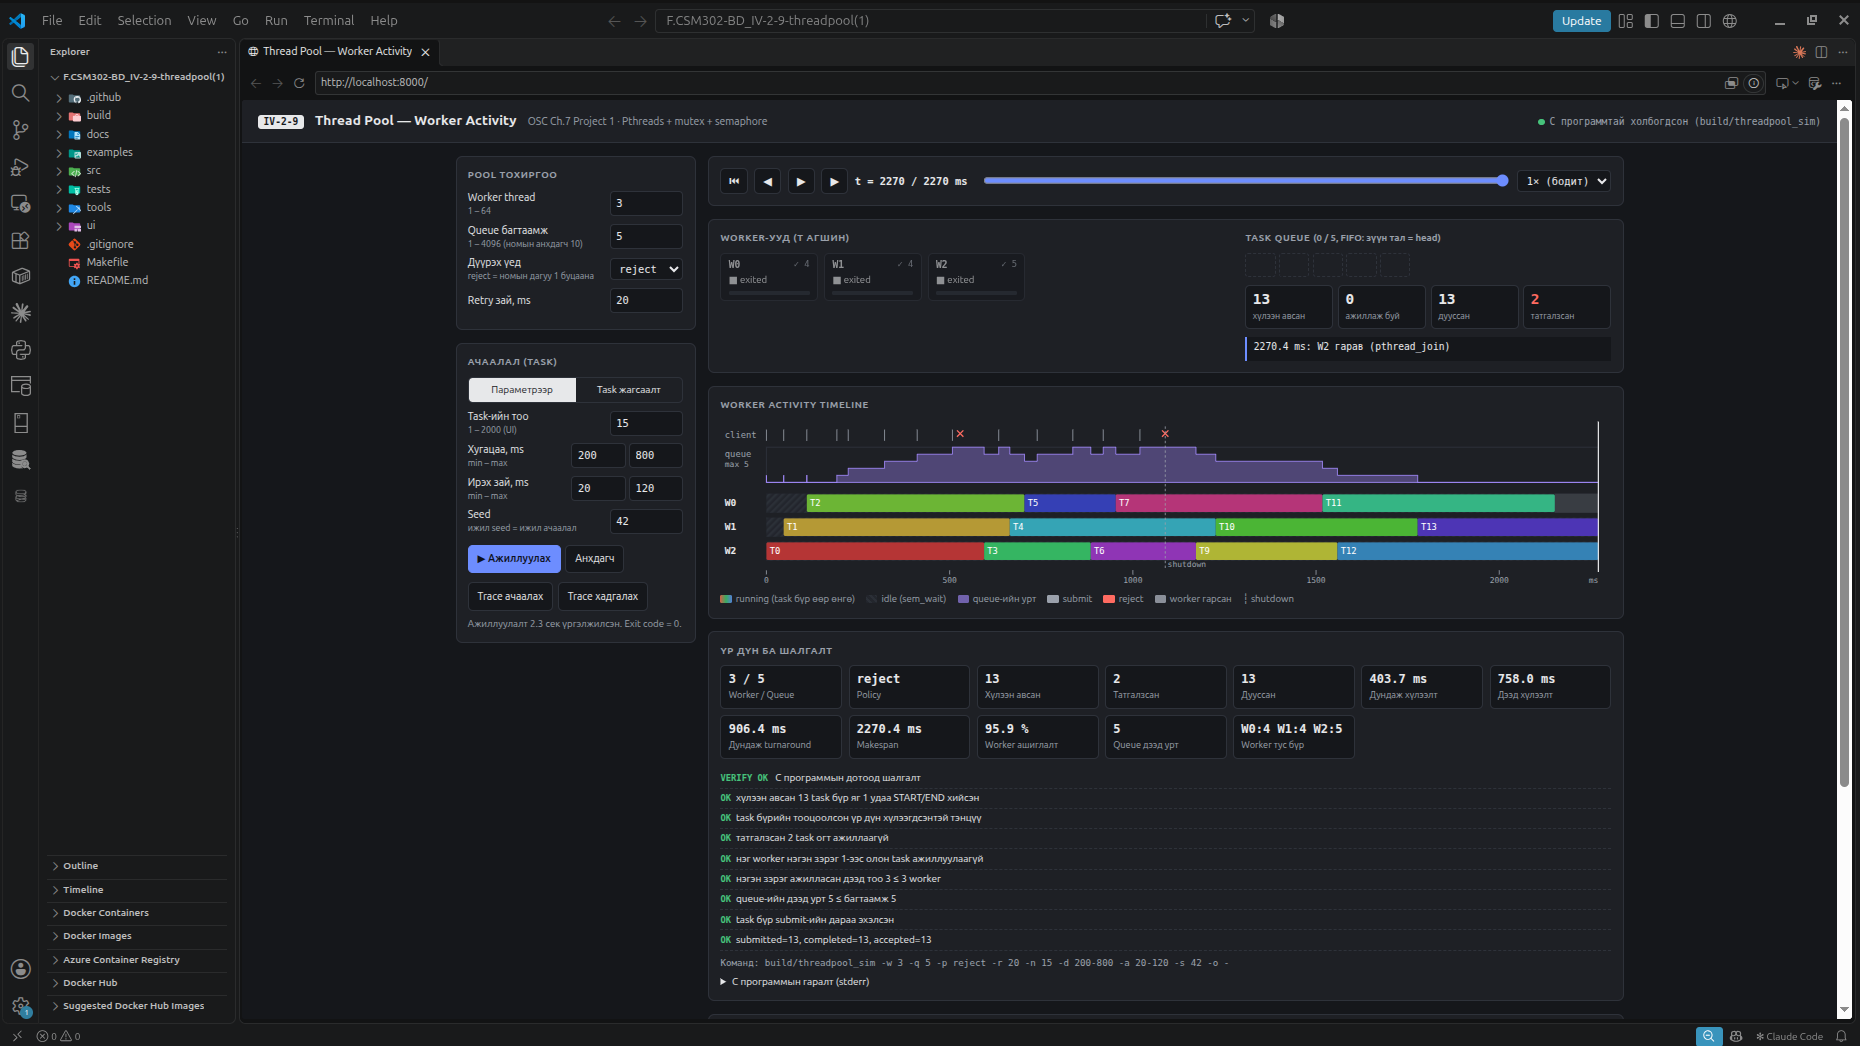
\includegraphics[width=1.00\linewidth]{img/user/ui_vscode_end.png}}}
\caption{Хэрэглэгчийн компьютер: VS Code-ийн browser дээр Worker activity, ажиллалтын төгсгөл (бүх worker exited, VERIFY OK)}\label{fig:uiend}
\end{figure}

Зураг \ref{fig:uilog}-д playback-ийг \code{t = 2137 ms} агшинд зогсоосон: W0, W1, W2 нь T11, T13, T12-ийг гүйцэтгэж (running), queue хоосон, 10 task дууссан. Доорх терминалд \code{make ui}-ийн серверийн бүртгэл харагдана: браузер \code{GET /}, \code{/api/health}, \code{/api/presets} хүсэлтийн дараа \code{POST /api/run} илгээж, сервер C программыг ажиллуулаад 200 кодоор trace буцаасан. Өөрөөр хэлбэл дэлгэцийн дүрслэл бодит C программын ажиллалтаас гарсан. \code{/favicon.ico}-ийн 404 нь хуудасны дүрс тэмдэг байхгүйг заах бөгөөд ажиллагаанд нөлөөлөхгүй.

\begin{figure}[H]
\centering
{\setlength{\fboxsep}{0pt}\setlength{\fboxrule}{0.5pt}\fcolorbox{frameline}{white}{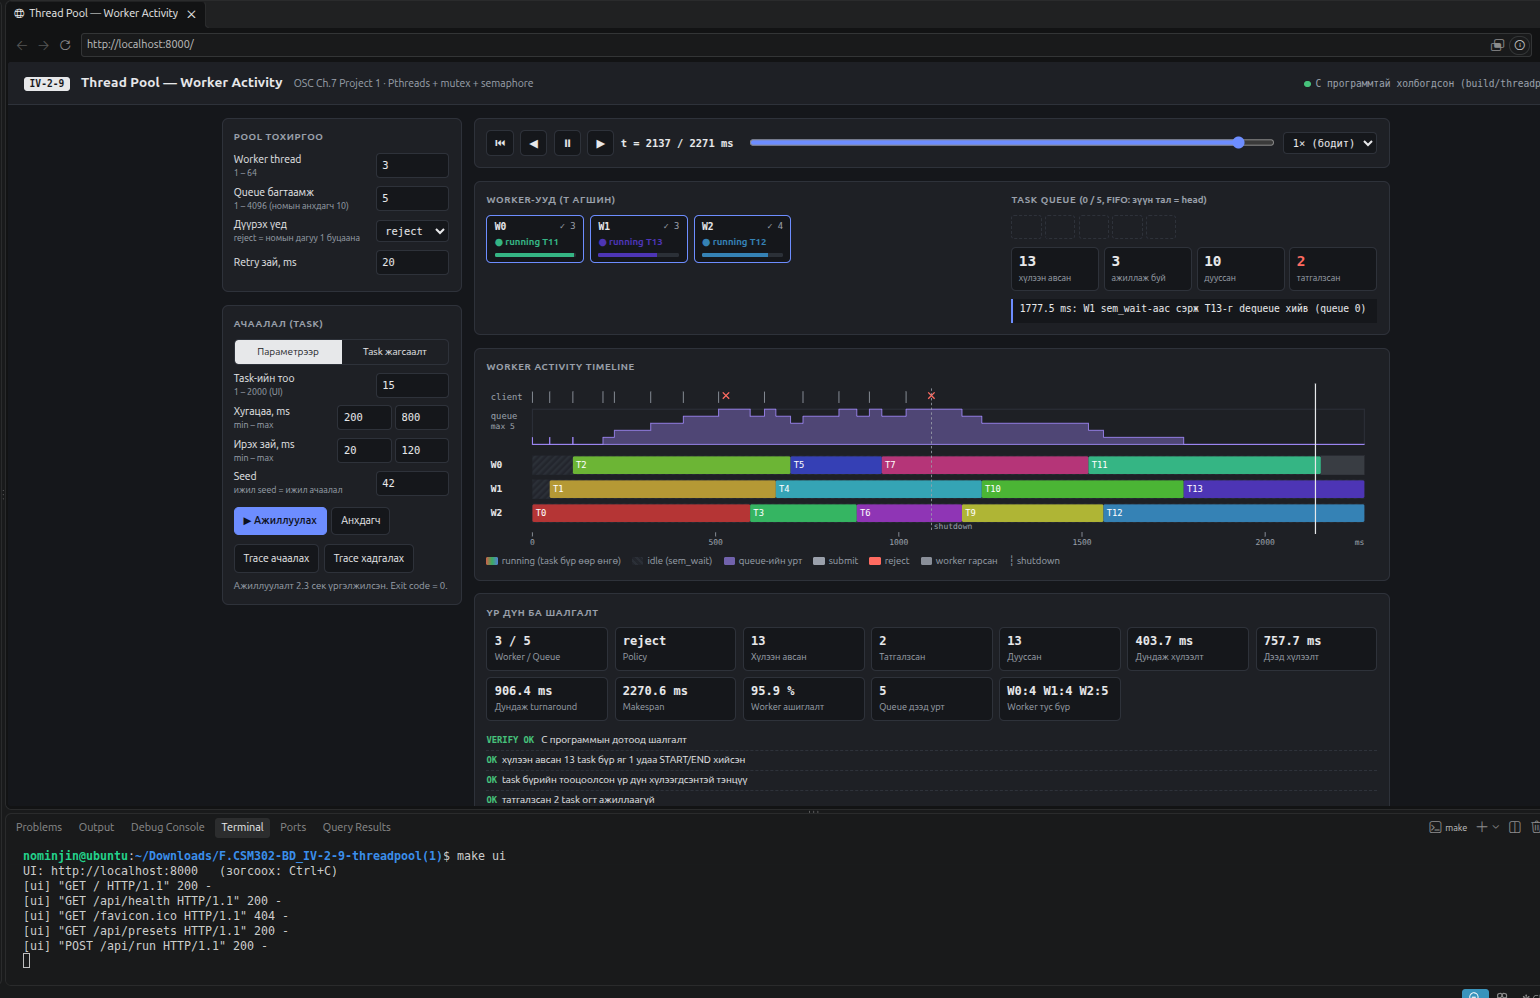
\includegraphics[width=1.00\linewidth]{img/user/ui_running_server_log.png}}}
\caption{Ажиллалтын дунд агшин (3 worker running) ба серверийн бүртгэл (POST /api/run 200)}\label{fig:uilog}
\end{figure}

Зураг \ref{fig:utest}-д \code{make test}-ийн бүрэн гаралт: номын жишээ, 6 үндсэн, 5 захын тест бүр C талын шалгалт болон хараат бус trace шалгагчаар ("trace шалгалт: OK") баталгаажиж, 17 буруу оролтын тест бүр зөв алдааны мессеж өгсөн. Төгсгөлд \code{Нийт: 29 PASS, 0 FAIL}. Тоон утгууд (хүлээлт, ашиглалт) Хүснэгт \ref{tab:tests}-ийнхтэй ойролцоо, хүлээн авсан/татгалзсан тоо ижил.

\begin{figure}[H]
\centering
{\setlength{\fboxsep}{0pt}\setlength{\fboxrule}{0.5pt}\fcolorbox{frameline}{white}{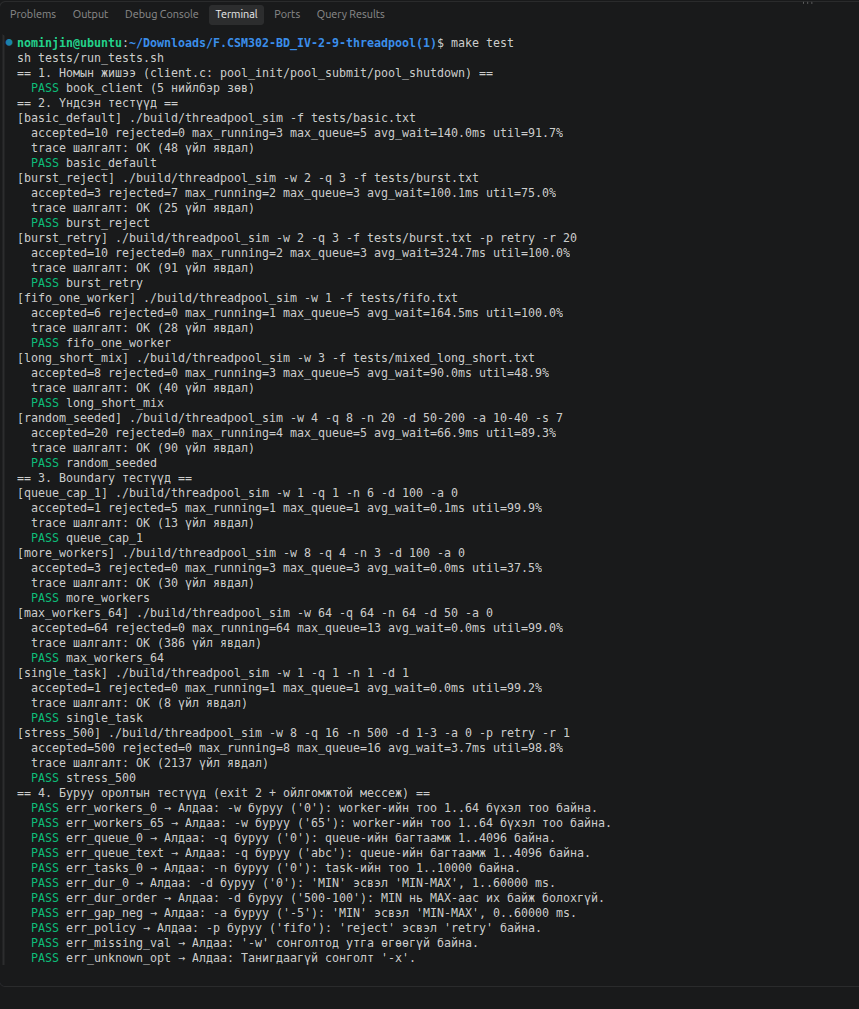
\includegraphics[width=0.66\linewidth]{img/user/make_test_1.png}}}\\[2pt]
{\setlength{\fboxsep}{0pt}\setlength{\fboxrule}{0.5pt}\fcolorbox{frameline}{white}{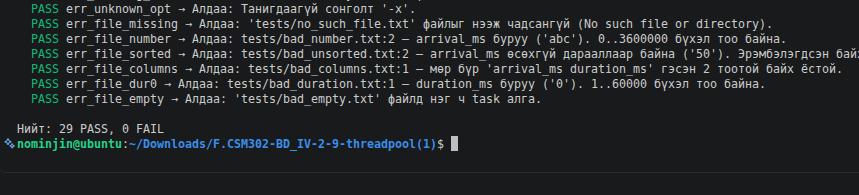
\includegraphics[width=0.66\linewidth]{img/user/make_test_2.png}}}
\caption{Хэрэглэгчийн компьютер дээрх make test: 29 PASS, 0 FAIL}\label{fig:utest}
\end{figure}

Зураг \ref{fig:ucli}-д серверийг \code{Ctrl+C}-ээр зогсоосны ("Сервер зогслоо") дараа CLI командуудыг шууд ажиллуулсан. \code{./build/client}-ийн 5 нийлбэр зөв боловч хэвлэгдсэн дараалал (3, 0, 42, 15, 300) өмнөх ажиллалтаас (15, 3, 300, 0, 42) өөр байна. Энэ нь гурван worker зэрэгцэн ажиллаж, аль нь түрүүлж дуусахыг OS scheduler шийддэгийн бодит жишээ бөгөөд алдаа биш. \code{-w 3 -q 5 -n 15} ажиллалтад 15 task бүгд гүйцэтгэгдэж, burst тестэд queue (3) дүүрч 7 task татгалзагдсан нь номын "дүүрвэл 1 буцаана" дүрмийг харуулна. Төгсгөлд \code{-h} нь бүх сонголтын тайлбарыг хэвлэв.

\begin{figure}[H]
\centering
{\setlength{\fboxsep}{0pt}\setlength{\fboxrule}{0.5pt}\fcolorbox{frameline}{white}{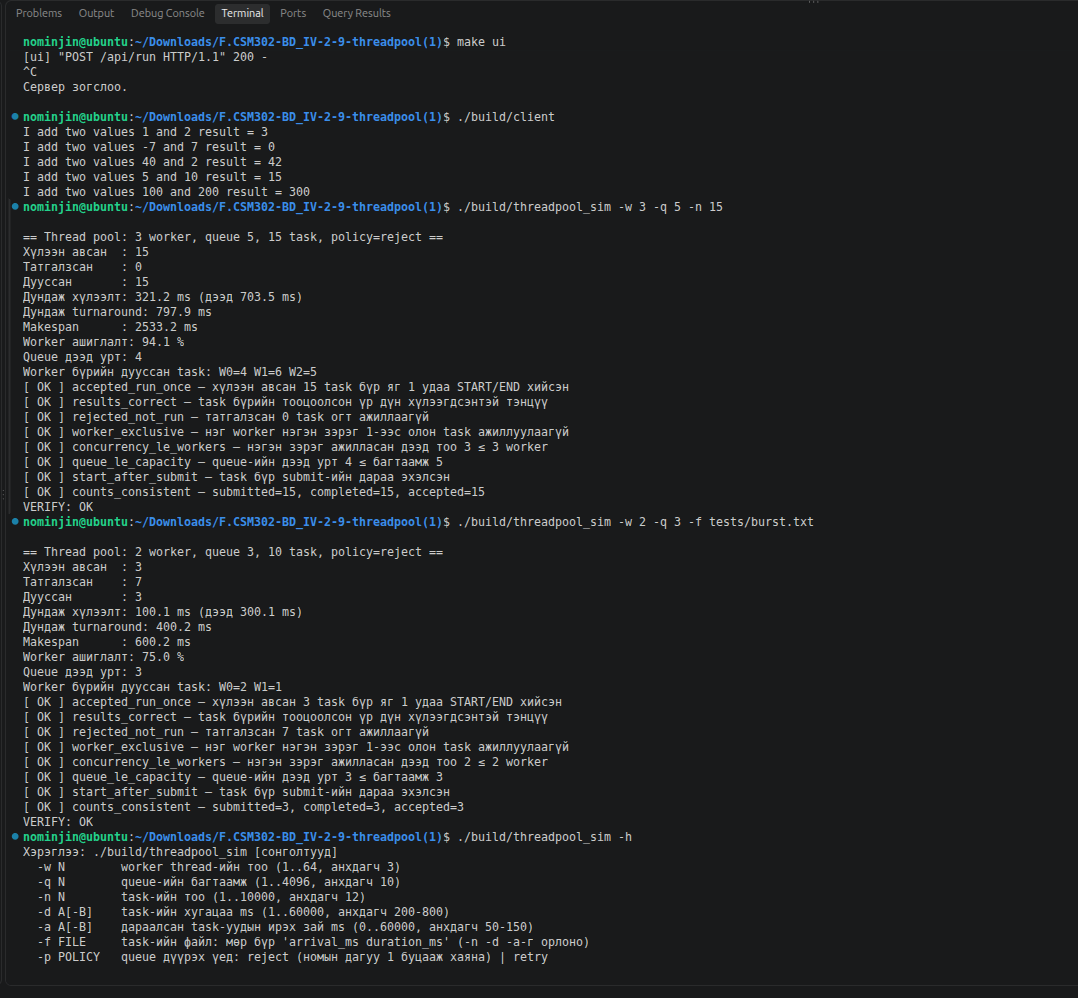
\includegraphics[width=0.82\linewidth]{img/user/client_sim_cli.png}}}
\caption{Серверийг зогсоох, номын client.c, анхдагч ба burst ажиллалт, -h тусламж}\label{fig:ucli}
\end{figure}

Зураг \ref{fig:utsan}-д \code{make tsan}: программыг \code{-fsanitize=thread}-тэй хөрвүүлж, 4 worker, queue 3, 40 task-ийг retry горимоор маш богино (5-30 мс) хугацаатай ажиллуулсан. Queue байнга дүүрч client 58 удаа дахин оролдсон ч ThreadSanitizer нэг ч \code{WARNING} гаргаагүй, 40 task бүр яг нэг удаа гүйцэтгэгдэж \code{VERIFY: OK}. Энэ нь өрсөлдөөн ихтэй нөхцөлд ч mutex болон semaphore queue-г зөв хамгаалж байгааг баталгаажуулна.

\begin{figure}[H]
\centering
{\setlength{\fboxsep}{0pt}\setlength{\fboxrule}{0.5pt}\fcolorbox{frameline}{white}{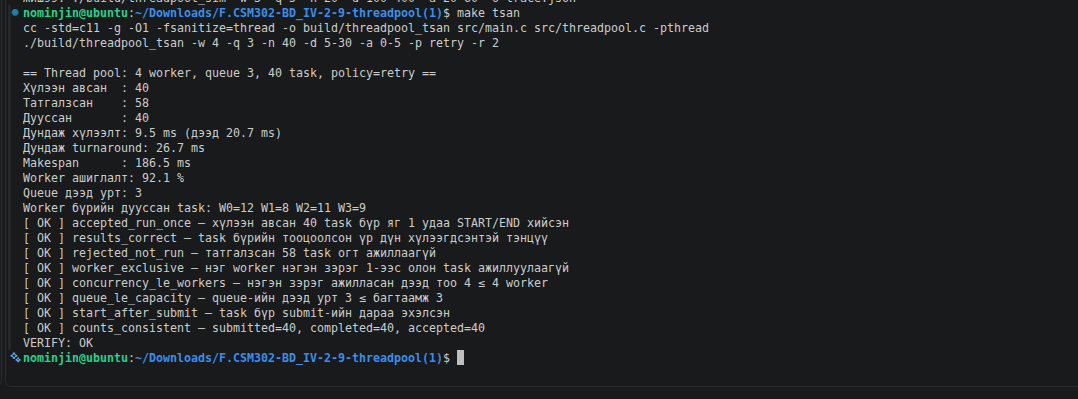
\includegraphics[width=0.82\linewidth]{img/user/make_tsan.png}}}
\caption{Хэрэглэгчийн компьютер дээрх ThreadSanitizer: race илрээгүй, VERIFY OK}\label{fig:utsan}
\end{figure}

% ======================================================================
\section{Хэлэлцүүлэг}

\subsection{Үр дүнгийн тайлбар}

Бүх тестэд, тэр дундаа 64 worker зэрэг ажилласан болон 500 task-ийн stress нөхцөлд task бүр яг нэг удаа ажиллаж, нэг worker давхар task аваагүй, queue FIFO-оор ажиллаж, багтаамжаас хэтрээгүй нь mutex queue-ийн өгөгдлийг, semaphore task-ийн тоог зөв хамгаалж байгааг харуулна. Idle worker-ууд \code{sem\_wait} дээр унтдаг тул CPU үрэхгүй; timeline-ийн судалтай саарал бүс тэдгээрийн бодит хүлээлт юм. Task-ууд \code{nanosleep} хийдэг (I/O-той адил) учраас worker-ийн тоо CPU-ийн цөмийн тооноос олон байсан ч хурдатгал бараг шугаман хэвээр байсан.

Ижил параметрээр дахин ажиллуулахад аль worker аль task-ийг авах, burst үед хэдэн task хүлээн авагдах нь бага зэрэг өөрчлөгдөж болно (T3: 3-5). Энэ нь OS scheduler-ийн шийдвэр бөгөөд тест ийм хэлбэлзлийг мужаар шалгадаг.

\subsection{Хүлээх дараалал ба deadlock}

Worker эхлээд \code{sem\_wait}, дараа нь \code{pthread\_mutex\_lock} хийх ёстой. Хэрэв дарааллыг солиод mutex-ийг барьсан чигээр хоосон queue дээр \code{sem\_wait} хийвэл client mutex авч чадахгүй, task нэмэгдэхгүй тул хэн ч урагшлахгүй (deadlock). Мөн client \code{sem\_post}-ийг mutex суллагдсаны дараа хийдэг. Mutex-ийг зөвхөн queue-г өөрчлөх богино хэсэгт барьж, task-ийг гүйцэтгэх болон хүлээлтийг critical section-ээс гадуур хийсэн.

\subsection{Хязгаарлалт}

\begin{itemize}
  \item Task-ийн ажлыг \code{nanosleep}-ээр дуурайлгасан (номын зөвлөмж). CPU-д ачаалалтай ажилд хурдатгал цөмийн тоогоор хязгаарлагдана.
  \item Trace бүртгэл тусдаа mutex ашигладаг тул маш богино (< 1 мс) task-уудад бага зэргийн нэмэлт зардал үүсгэнэ.
  \item Нэг client thread submit хийдэг; retry горимд түүний хүлээлт дараагийн task-уудын ирэлтийг хойшлуулна.
  \item Номын API глобал төлөвтэй тул нэг процесст нэг pool ажиллана.
  \item Интерфейсийн хязгаар (2000 task, \textasciitilde{}60 с) C программынхаас (10000 task) нарийн.
\end{itemize}

% ======================================================================
\section{Дүгнэлт}

Сурах бичгийн Programming Project 1-ийг C хэл, pthreads, POSIX semaphore, mutex ашиглан бүрэн хэрэгжүүлж, worker-ийн тоо, queue-ийн багтаамж, дүүрэх үеийн бодлого, ачааллыг өөрчилж турших боломжтой болгосон. Номын \code{client.c} жишээ өөрчлөлтгүй ажиллав. Багшийн оноосон "Worker activity" дүрслэлийг бодит программын trace-тэй шууд холбож, worker бүрийн idle, running, completed төлөв, queue, татгалзлыг алхам алхмаар харуулав. 29 автомат тест, хараат бус trace шалгагч, ThreadSanitizer зөв ажиллагааг нотолж, гүйцэтгэлийн туршилт worker нэмэхэд хурдатгал бараг шугаман байгааг харуулсан. Manual-ын дагуу \code{make}, \code{make ui} гэсэн хоёр командаар өөр компьютерт ажиллуулах боломжтой.

\section*{Ашигласан материал}
\addcontentsline{toc}{section}{Ашигласан материал}

\begin{enumerate}[label={[\arabic*]}, leftmargin=2.4em]
  \item A. Silberschatz, P. B. Galvin, G. Gagne. \textit{Operating System Concepts}, 10th ed. Wiley, 2018. 4.5.1 (Thread pools), 4.6.3 (Thread cancellation), 6.5–6.6, 7.1.1, 7.3; Chapter 7 Programming Project 1 "Designing a Thread Pool".
  \item The Open Group. POSIX.1-2017: \code{pthread\_create}, \code{pthread\_join}, \code{pthread\_mutex\_lock}, \code{sem\_init}, \code{sem\_wait}, \code{sem\_post}.
  \item Linux man-pages: \code{sem\_overview(7)}, \code{pthreads(7)}, \code{nanosleep(2)}.
  \item ThreadSanitizer. \url{https://clang.llvm.org/docs/ThreadSanitizer.html}
  \item F.CSM302 Бие даалт 1 удирдамж, Сэдэв ба шүүмжийн хуваарилалт.
  \item Багийн repository. \url{github.com/NominjinNomio/F.CSM302-BD_IV-2-9-threadpool}
\end{enumerate}

\clearpage
\section*{Хавсралт А. Ажлын төлөвлөгөө}
\addcontentsline{toc}{section}{Хавсралт А. Ажлын төлөвлөгөө}

\begin{table}[H]
\centering
\begin{tabular}{|P{0.300}|P{0.700}|}
\hline
\rowcolor{tablehead} \textbf{Талбар} & \textbf{Мэдээлэл} \\ \hline
Хуваарилалтын код & IV-2-9 \\ \hline
Төсөл & Designing a Thread Pool \\ \hline
Repository & \url{https://github.com/NominjinNomio/F.CSM302-BD_IV-2-9-threadpool} \\ \hline
Хэл/сан/орчин & C (pthreads, POSIX semaphore), Python 3, HTML/JavaScript; Linux, macOS, WSL2 \\ \hline
Үндсэн дүрслэл & Worker activity \\ \hline
\end{tabular}
\end{table}

\begin{table}[H]
\centering
\begin{tabular}{|P{0.240}|P{0.460}|P{0.300}|}
\hline
\rowcolor{tablehead} \textbf{Гишүүн} & \textbf{Хариуцах ажил} & \textbf{Commit/file} \\ \hline
Ц.Номинжин\newline /B241940137/ & Сервер, CI, screenshot & \code{tools/, .github/} \\ \hline
Ц.Номинжин\newline /B241940137/ & Туршилтын программ, CLI, оролтын шалгалт & \code{src/main.c, examples/} \\ \hline
Ц.Номинжин\newline /B241940137/ & Автомат тест, trace шалгагч, туршилт & \code{tests/} \\ \hline
Ц.Номинжин\newline /B241940137/ & Thread pool core: queue, mutex, semaphore, worker & \code{src/threadpool.c, src/threadpool.h} \\ \hline
Ц.Номинжин\newline /B241940137/ & Worker activity интерфейс & \code{ui/index.html} \\ \hline
Ц.Номинжин\newline /B241940137/ & Тайлан, гарын авлага & \code{docs/, README.md} \\ \hline
\end{tabular}
\end{table}

\begin{table}[H]
\centering
\begin{tabular}{|P{0.100}|P{0.450}|P{0.450}|}
\hline
\rowcolor{tablehead} \textbf{Тест} & \textbf{Оролт/нөхцөл} & \textbf{Хүлээгдсэн үр дүн} \\ \hline
1 & \code{./build/client} (номын жишээ) & 5 нийлбэр зөв \\ \hline
2 & W=3, Q=10, basic.txt & 10/10 хүлээн авна, зэрэг ≤ 3 \\ \hline
3 & W=2, Q=3, burst.txt (queue дүүрэх) & 3-5 хүлээн авна, үлдсэнд \code{pool\_submit} 1 буцаана \\ \hline
4 & W=1, fifo.txt & FIFO дараалал \\ \hline
5 & W=0, буруу файл & exit 2, алдаатай утга/мөрийг заасан тайлбар \\ \hline
\end{tabular}
\end{table}

\end{document}
